% \documentclass[A4, 12pt]{article}
\documentclass{article}

% Page setup
\usepackage[a4paper, margin=1in]{geometry}

% Spacing and indentation
\usepackage{setspace}
\setlength{\parindent}{0.5in} 
\setlength{\parskip}{0pt} 
\doublespacing


% Math and graphics
\usepackage{graphicx}
\usepackage{amsmath}

% Tables
\usepackage{multirow}
\usepackage{booktabs}
\usepackage{float}


% Bibliography
\usepackage[backend=biber,style=apa]{biblatex}
% \addbibresource{/home/pnx/Documents/sp_env/sp_latex_source/rrl.bib}

\usepackage{titlesec}
\usepackage{titletoc}


\titleformat{\section}[block]
  {\normalfont\Large\bfseries\centering}
  {\MakeUppercase{Chapter \thesection}}{0pt}{\\\MakeUppercase}


\title{Interpretable Deep Learning: Shapley-based Analysis of Generative Models for Synthetic Data Generation}
\begin{document}
% \author{Pinky Grace A. Marfa}
% \date{January 1, 2025}



% \begin{titlepage}
%     \centering
%     
\includegraphics[height=3cm]{assets/up-logo2.jpg}
%     
\includegraphics[height=3cm]{assets/upc-logo.jpeg} \\ [0.5cm]

%     \Large \textbf{Interpretable Deep Learning: Shapley-based Analysis of Generative Models for Synthetic Data Generation} \\ [0.2cm]
%     \rule{\textwidth}{0.1pt}

%     \large A Special Project Presented to the \\
%     \large Faculty of the Department of Computer Science, \\
%     \large College of Science, \\
%     \large University of the Philippines Cebu\\
%     \vfill
%     \large In Partial Fulfillment \\
%     \large Of the Requirements for the Degree \\
%     \large Bachelor of Science in Computer Science \\
%     \rule{\textwidth}{0.1pt}
%     \vfill
%     \large Pinky Grace A. Marfa \\
%     \large Bachelor of Science in Computer Science \\
%     \vfill
%     \large Asst. Prof. Dharyll Prince M. Abellana \\
%     \large Special Problem Adviser \\
%     \vfill
%     \large January 2025
% \end{titlepage}

% \maketitle

\pagenumbering{roman}
\thispagestyle{empty}

\newpage

\begin{center}
\Large\textbf{ACKNOWLEDGEMENTS}
\end{center}

\vspace{1em} % adds a little vertical space

\newpage

\begin{center}
\Large\textbf{DEDICATION}
\end{center}

\vspace{1em} % adds a little vertical space

\newpage

\begin{center}
\Large\textbf{Abstract}
\end{center}

\vspace{1em} % adds a little vertical space

\newpage
% Add after \tableofcontents
\tableofcontents
\thispagestyle{empty} % Remove page number from TOC page
\newpage

\pagenumbering{arabic}
\setcounter{page}{1}
\section{INTRODUCTION}

\subsection{Rationale}
The increasing reliance on machine learning (ML) models across various domains such as healthcare, finance, and cybersecurity has fueled an increasing demand for high-quality data that can be used to train and test these systems. However, access to real-world data often comes with significant challenges, including privacy concerns, data scarcity, and algorithmic biases. In recent years, synthetic data generation has emerged as a viable solution to these challenges.

While synthetic data provides a promising alternative to real-world data, its effectiveness largely relies on its quality, which can be assessed based on fidelity and usability. Fidelity evaluates how closely the synthetic data replicates the statistical properties of the original data, while usability assesses its efficacy in supporting ML tasks. These dimensions are interdependent: high fidelity ideally enhances usability, assuming the original data is reliable. However, if the original dataset contains flaws or biases, replicating it with high fidelity might only perpetuate its limitations. Thus, it is essential for synthetic data to not simply mimic the original data but also address and improve upon its deficiencies to ensure greater usability.

This study aims to evaluate and compare the effectiveness of various generative models in producing synthetic datasets that are both statistically similar to real data (high fidelity) and practically useful in ML applications (high usability). The ultimate goal is to identify models that can best mitigate the shortcomings of low-quality datasets, thereby enhancing the overall robustness and reliability of machine learning systems. Utilizing a Shapely-based analysis, this research quantitatively assesses each generative model’s contribution to the quality of synthetic data. This comprehensive evaluation seeks to determine each model’s capability not only to adhere closely to the statistical properties of the original data but also to enhance the effectiveness of downstream ML applications. By dissecting the contributions of Generative Adversarial Networks (GANs), Variational Autoencoders (VAEs), and their combined applications in time series data generation, the study aims to pinpoint which models provide the optimal balance between fidelity and usability.

\subsection{Statement of the Problem}
Generative models, including GANs, VAEs, and their hybrids, have demonstrated significant potential in addressing data scarcity and privacy concerns through synthetic data generation. However, the effectiveness of these models in producing high-quality synthetic time series data, particularly when evaluated against the dual metrics of fidelity and usability, remains underexplored. Synthetic data must not only mimic the statistical properties of the original datasets but also support effective machine learning applications—a dual requirement that poses significant challenges, especially when the original data is flawed.

This leads to a notable research gap: there is no established and robust methodology for evaluating which generative models best navigate the trade-offs between fidelity and usability in time series data applications. Addressing this gap, this study employs a Shapely-based analysis to systematically compare these models. This innovative approach will help identify which models not only balance fidelity and usability effectively but also produce synthetic data of a quality that significantly enhances the robustness and reliability of machine learning systems. Such insights are crucial for advancing the use of synthetic datasets, particularly in environments where high-quality real data is scarce or privacy concerns restrict its use.

\subsubsection{Research Questions}
\begin{enumerate}
    \item How can fidelity and usability metrics be effectively integrated into a comparative evaluation of generative models for time series synthetic data generation?
    \item What trade-offs exist between fidelity and usability in synthetic data generation, and how do these trade-offs affect downstream machine learning tasks?
    \item Which generative model most effectively balances fidelity and usability to produce high-quality synthetic time series data?
\end{enumerate}

\subsection{Significance of the Study}
This study addresses a critical gap in the literature on synthetic data generation, particularly focusing on the balance between fidelity and usability in datasets generated for time series applications. While generative models like GANs, VAEs, and their hybrids have shown promise in isolated studies, there remains a substantial need for a comprehensive evaluation framework that assesses these models based on their ability to produce high-quality synthetic datasets.

By applying a Shapely-based analysis, this study provides a systematic approach for assessing how well synthetic data supports machine learning tasks while maintaining statistical similarity to real data. This dual-focus approach is crucial because generating high-quality synthetic data requires more than mere replication of the original data’s statistical features; it must also enhance the data's practical utility for machine learning tasks, particularly when the original datasets are flawed or biased.

The outcomes of this study are expected to significantly impact the field by providing actionable insights that can guide the development and refinement of generative models. Identifying models that effectively balance these two critical dimensions will help researchers and practitioners in fields where the quality of synthetic data is particularly important for overcoming challenges like data scarcity and bias without sacrificing the data’s utility.

\subsection{Scopes and Delimitations of the Study}
This study focuses on evaluating the quality of synthetic data generated by specific generative models—Generative Adversarial Networks (GANs), Variational Autoencoders (VAEs), and their hybrid—within the context of time series applications. The primary evaluation framework integrates the concept of fidelity and usability. These two concepts are treated as interrelated aspects of data quality, rather than as separate, isolated evaluative criteria.

\subsubsection{Delimitations}
\begin{itemize}
    \item \textbf{Privacy Metrics:} While privacy is crucial for synthetic data, especially in regulated fields, this study excludes privacy metrics to maintain a clear focus on evaluating synthetic data quality through fidelity and usability. Integrating privacy metrics would broaden the scope of the research and require more complex methodologies, such as differential privacy techniques, which would complicate the evaluation process and possibly overshadow the evaluation of the other metrics. The exclusion of privacy metrics allows this research to provide a more concentrated and detailed analysis of how well synthetic data replicates statistical properties and supports machine learning tasks. By focusing exclusively on fidelity and usability, the study aims to offer deeper insights into the core aspects of synthetic data quality without the confounding effects of integrating privacy considerations, which could be addressed in future research.

    \item \textbf{Generative Models:} The study limits its analysis to GANs, VAEs, and their hybrid GAN-VAEs. Other types of generative models, such as Restricted Boltzmann Machines or Diffusion Models, are not included in this assessment. This delimitation is based on the established capability of the selected models to handle time series data effectively, which is central to the research questions posed.

    \item \textbf{Dataset Size:} To manage computational costs and training time, the study employs datasets standardized to contain a maximum of 3,900 samples. This ensures consistent and efficient evaluation across all models without compromising the integrity of the results.
    
    \item \textbf{General Applications:} The study focuses on general synthetic data generation for time series applications and is not tailored to specific domains such as healthcare or finance. While the methods used in this research could be adapted for domain-specific applications, the findings are intended to provide insights that are broadly applicable.

    \item \textbf{Evaluation Focus:} The study does not aim to separately optimize fidelity and usability metrics but rather examines the balance and trade-offs between them in producing high-quality synthetic data. This approach is chosen to better understand how improvements in one aspect might affect the other, providing a holistic view of model performance. 

\end{itemize}

\subsubsection{Limitations}
\begin{itemize}
    \item \textbf{Dataset Representation:} The findings are limited to the datasets used in this study, which include time series datasets of varying dimensionality.  These datasets, selected for their relevance to existing literature and practicality, may not fully represent the diversity and complexity of real-world time series data.

    \item \textbf{Evaluation Scope:} The evaluation is limited to forecasting tasks using LSTM as the downstream application for utility assessment, which may not generalize to other machine learning tasks such as classification or clustering.
    
    \item \textbf{Computational Constraints:} The decision to limit dataset size and use simpler forecasting models, such as Multiple Linear Regression, reflect practical constraints and may not capture the full potential of generative models under larger-scale experiments.

    \item \textbf{Exclusion of Privacy Metrics: } While privacy metrics are not included in this study, their absence represents a potential area for future exploration. This limitation reflects a deliberate decision to focus on fidelity and usability, which are critical dimensions of synthetic data quality. Privacy-preserving synthetic data generation is only meaningful if the synthetic data itself has high fidelity and usability. By ensuring that the foundation of synthetic data quality is addressed first, this study creates a strong basis for exploring privacy considerations in future work. However, the exclusion of privacy metrics means this study does not evaluate the extent to which the generated datasets mitigate risks of privacy breaches, leaving this as an area for further exploration.

\end{itemize}


\newpage
\section{Literature Review}

\subsection{Overview of Synthetic Data Generation}

Synthetic data refers to artificially generated data produced through specialized mathematical models or algorithms, specifically designed to address particular data science tasks (Jordon et al, 2022). According to Jordon et al. (2022), synthetic data serves as a tool to address various challenges in data science, including privacy concerns, bias, and data scarcity, without directly exposing sensitive information. This view is further supported by Goyal and Mahmoud (2024) who have highlighted the increasing recognition of synthetic data for its potential to address pressing real-world issues such as mitigating data scarcity, addressing privacy concerns, and reducing algorithmic biases— issues common in machine learning applications. Similarly, El Emam et al. (2020) emphasizes that although it is not real data, synthetic data is generated based on the statistical properties of the original dataset, ensuring it mirrors the original data in terms of patterns and distributions. This approach enables for the preservation of statistical integrity while mitigating risks related to data privacy breaches.  

Expanding on these definitions, synthetic data has seen widespread adoption in a variety of fields, where the aforementioned challenges are most pronounced. This is especially evident in the healthcare domain, where access to relevant datasets is often constrained due to privacy and scarcity. A study by Skandarani et al. (2021) illustrates this through the use of Generative Adversarial Networks (GANs) to generate medical images to enable meaningful research. This application is further elaborated by Habiba et al (2021), who investigated ECG synthesis using Neural Ordinary Differential Equations (ODE) and GAN models, demonstrating another facet of how synthetic data can support advancements in medical research. Similarly, in other domains like finance, where there is a need for balanced datasets and anonymization, synthetic data has proven beneficial as exemplified by Caliskan et al. (2023), comparatively analyzing the Variational Auto-Encoder (VAE) and Conditional Tabular Generative Adversarial Network (CTGAN) for generating synthetic financial credit load data. Additionally, synthetic data is also used in network traffic simulation (Cullen et al, 2022), supporting cybersecurity applications through the generation of anonymized datasets.

Despite its utility, there remains significant open challenges in the field of synthetic data generation. A recurring theme across the related literature is the lack of well-agreed metrics for evaluating the quality, utility, and privacy of synthetic data (Goyal and Mahmoud, 2024; Caliskan et al., 2023); Bauer et al., 2024; Lu et al., 2023). This absence of well-agreed evaluation methods makes it a challenging task to compare the performance of different models, such as GANs, VAEs, and Neural ODEs, and to determine which model is best suited for a given application, as observed in a systematic review by Goyal and Mahmoud (2024). For example, while some studies rely on statistical difference evaluations like Kullback-Leibler (KL) divergence or Wasserstein distance (Li et al., 2019), others employ human evaluation or application-specific metrics to assess synthetic data quality (Lu et al., 2023), which further contributes to the inconsistencies in evaluation. Beyond evaluation, the balance between fidelity and privacy also remains a critical issue, with multiple studies emphasizing the difficulty of generating data that mirrors the original dataset while protecting sensitive information (Goyal and Mahmoud, 2024). Additional issues include propagation of biases (Jordon et al, 2022), fairness issues (Lu et al., 2023), high computational costs (Bauer et al., 2024) and the lack of robust privacy-preserving techniques (Kaabachi et al., 2023).

In light of the challenges discussed above, it is evident that the field of synthetic data generation is at a crucial juncture. Given the growing reliance on machine learning models across sectors, understanding how to measure the quality and impact of synthetic data will become increasingly important. Thus, the study of metrics for evaluating synthetic data—in terms of both privacy protection and data utility—will be a critical area of future research. Such metrics will not only improve synthetic data's applicability across industries but also enhance trust in its use for privacy-sensitive applications like healthcare and finance.

\subsection{Metrics for Evaluating Synthetic Data}

As the field of synthetic data generation evolves, the need for robust and widely-accepted metrics to evaluate the quality, utility, and privacy of synthetic data has become increasingly apparent. These metrics are essential not only for ensuring that synthetic data serves practical purposes but also for guaranteeing its ethical use in sensitive applications such as healthcare (Kaabachi et al., 2023). Evaluation metrics are crucial for determining how well synthetic data replicates the original dataset while maintaining privacy, ensuring the data’s usability, and avoiding unintended consequences such as the leakage of sensitive information (Jordon et al, 2022; Kaabachi et al., 2023). In the literature, synthetic data evaluation metrics are broadly categorized into two categories: utility metrics and privacy metrics (Goncalves et al., 2020; Kaabachi et al., 2023). 

Utility metrics play a key role in assessing how well synthetic data retains the essential characteristics of the original data, ensuring its usefulness for tasks such as machine learning model training and data analysis. As defined by Hittmeir et al. (2019), utility metrics quantify how useful synthetic data is by assessing how much information is lost during the data generation process.  In this way, they help determine how closely the synthetic data mirrors the original, supporting its use in real-world applications. These utility metrics can be further divided into general and task-specific metrics (Kaabachi et al., 2023; Osorio-Marulanda et al, 2024).

General utility metrics assess the overall statistical properties and model evaluation results for a wide range of potential analyses that could be performed on the data (El Emam, 2020). These metrics focus on preserving key statistical attributes of the original dataset, such as the distribution of variables, means, variances, and correlations. Commonly used general utility metrics include KL Divergence and Wasserstein Distance, both of which measure the similarity between the probability distributions of the real and synthetic data (Fonseca \& Bacao, 2023). While general utility metrics provide a broad assessment of how well synthetic data mirrors the statistical properties of the original dataset, task-specific utility metrics evaluate synthetic data based on how well it supports specific tasks, such as machine learning applications. These metrics focus on the performance of models trained on synthetic data when applied to real-world tasks. Common task-specific utility metrics used in research include machine learning efficacy metrics like accuracy, precision, recall, and F1-score (Figueira \& Vaz, 2022. This approach is particularly useful in classification tasks, where the goal is to determine whether the synthetic data can be used to train models that perform comparably to those trained on real data (Kaabachi et al., 2023). 

In addition to utility metrics, privacy metrics are crucial for evaluating the extent to which synthetic data protects sensitive information in the original dataset. Differential Privacy (DP) is one of the most widely recognized privacy metrics, providing a formal framework that quantifies the privacy guarantees of a data release mechanism (Jordon et al, 2022; Goyal \& Mahmoud, 2024; Kaabachi et al., 2023; Nikolenko, 2019) . Similarly, Distance to Closest Record (DCR) offers another valuable perspective by measuring the distance between each synthetic data point and its nearest neighbor in the real training dataset (Mendelevitch, 2021).

In evaluating synthetic data generation, one of the most significant challenges is the inconsistency in comparative evaluations of different methods, which arises from the lack of uniform evaluation metrics (Chundawat et al., 2022). This inconsistency leads to confusion and variability in determining the effectiveness of synthetic data. As different models and applications prioritize various aspects, such as privacy, accuracy, or utility, establishing a common ground for evaluation becomes problematic. For example, while some methods may focus on enhancing privacy, others might aim to improve the accuracy or utility of the synthetic data, resulting in a diverse range of metrics that are not easily comparable. In response to these discrepancies, there have been concerted efforts within the research community to develop more unified evaluation metrics. One notable example is TabSynDex by Chundawat et al. (2022), a single-score metric designed to robustly evaluate synthetic tabular data. Another innovative metric that has been developed is SHAPr (2021), a Shapely-value based privacy metric which offers a versatile tool for measuring privacy risks.

However, these efforts encounter additional complexities. A prominent issue is the difficulty in balancing the trade-offs between privacy and utility. Enhancing privacy typically involves introducing mechanisms that may degrade the utility of the data by reducing its accuracy or limiting the types of analysis that can be performed effectively. This trade-off is particularly problematic in fields requiring high-fidelity data for accurate analysis, such as healthcare and finance, where both high utility and stringent privacy are critical (Mendelevitch, 2021; Caliskan et al., 2023). Moreover, many existing studies and methodologies fail to thoroughly evaluate residual privacy risks, especially concerning publicly released synthetic data (Kaabachi et al., 2023). This oversight can lead to significant privacy breaches, as residual information may still be exploited to uncover sensitive data about individuals in the original dataset. Lastly, the metrics currently employed often struggle to capture complex relationships and dependencies between multiple attributes in the data. This deficiency can lead to synthetic datasets that, while statistically similar to original datasets in marginal distributions, fail to preserve more complex interdependencies, thus limiting their usefulness for more sophisticated data science tasks (Jordon et al, 2022).

\subsection{Survey of Generative Deep Learning Models}

Generative deep learning models have emerged as powerful tools for creating synthetic data, increasingly becoming relevant in fields like healthcare, finance, and security, where data privacy and scarcity are major concerns. These models aim to capture the underlying data distribution of the training set in order to produce samples that reflect the learned distribution (Pati\~no \& Poll\'an, 2022). For example, GANs use an adversarial framework where the generator learns to model the data distribution by producing synthetic samples that fool a discriminator, which is trained to distinguish real from synthetic data. Similarly, VAEs utilize an encoder-decoder architecture, where the encoder maps data into a latent space and the decoder generates new samples by reconstructing data from this latent representation. Prior to the development of deep learning models, early generative approaches, such as Hidden Markov Models (HMMs) and Gaussian Mixture Models (GMMs) paved the way by capturing simple probabilistic relationships in data. However, as Cao et al. (2023) notes, it was the advent of deep learning that brought major performance advancements, allowing generative models to handle complex, high-dimensional data distributions. This idea is supported by Caliskan, Yayla, and Genc (2023), who suggest that the proliferation of deep learning algorithms and emergence of generative techniques offers more promising solutions in the generation of financial credit loan data. This leap in capability has established deep learning-based models as central to modern synthetic data generation. 

With the rise of deep learning, models such as GANs and VAEs have emerged as foundational generative models that leverage neural networks to capture and reproduce complex data distributions in high-dimensional spaces. GANs, introduced by Goodfellow et al. (2014), use an adversarial framework involving two neural networks, a generator and a discriminator. More specifically, the generator begins with random noise as its input and strives to produce data whose distribution challenges the discriminator’s ability to classify it as real or synthetic. Based on the discriminator’s classification results, the gradients of the generator are updated to better approximate the real data distribution (Zia et al., 2023). Although initially focused on synthetic image generation, GANs have extended their utility beyond image synthesis to domains like time-series data generation (Yoon et al., 2019). 

VAEs represent another class of generative models frequently used for synthetic data generation. Proposed by Kingma and Welling (2013), VAEs use a probabilistic approach, learning to encode input data into a latent space in a manner that enables controlled sampling. Unlike GANs, which rely on adversarial training, VAEs  employ a probabilistic approach using encoder and decoder networks to learn and generate data (Lu et al., 2024). One of the key strengths of VAEs lies in their ability to generate smooth, continuous latent spaces. This quality enables fine control over the generative process, allowing the user to manipulate specific features or generate data with particular attributes by sampling specific regions of the latent space, such as in anomaly detection (Niu et al., 2020), where VAEs can learn normal patterns and identify deviations as anomalies.

In addition to GANs and VAEs, Restricted Boltzmann Machines (RBMs) have also been critical in the evolution of generative models. Proposed by Salakhutdinov (2007), RBMs are models that can learn the distribution of the training data through a two-layer architecture — a visible layer that represents the observed data and a hidden layer that captures latent features (Pati\~no \& Poll\'an, 2022).  RBMs have been successfully applied in a range of tasks, including generating user preferences for recommendation systems like Netflix (Nematolahy, 2020) and reconstructing missing data in tabular datasets. For instance, in financial modeling, they have been used to generate synthetic market data, replicating the probability distributions of real-world datasets and capturing complex dependencies (Kondratyev \& Schwarz, 2019).

Originally introduced by Sohl-Dickstein et al. (2015), Diffusion Models have gained significant attention in synthetic data generation in recent years due to their ability to handle complex data distributions with stability and precision. As per Lin et al. (2023), the underlying principle of Diffusion Models is to progressively perturb observed data through a forward diffusion process and then recover the original data using a backward reverse process. The forward process involves multiple steps of noise injection, where the noise level changes incrementally at each step. Conversely, the backward process consists of a series of denoising steps, parameterized by a neural network, that gradually remove the injected noise. Once the backward process has been learned, Diffusion Models can generate new samples from almost any initial data (Lin et al., 2023). This is supported by a study by You et al. (2023) that highlights that Diffusion Models are particularly effective in scenarios with limited training data, as they can generate novel samples even when very few training samples are available. In addition, Zhu (2024) emphasizes that Diffusion Models, along with other foundational generative models like GANs, have become one of the most widely used methods for modeling the distribution of continuous-domain data and generating new samples. Their growing popularity reflects their versatility and robustness in a wide range of applications, especially as Diffusion Models have demonstrated their power over many existing generative techniques (Lin et al., 2023).

\newpage
\section{Methodology}
This study follows a structured methodological process that involves data preparation, evaluation of generative models, and analysis of their contributions to synthetic data quality. The focus is on assessing fidelity and usability metrics to determine which generative model provides the best balance between these dimensions. Each step is further elaborated in the following subsections.

\subsection{Dataset Preparation}
For this study, three multivariate datasets are considered. These datasets were chosen due to their widespread use in forecasting tasks in the literature, ensuring consistency and providing context for evaluating the generative models under study.

\begin{enumerate}
    \item \textbf{Exchange:} 
    
    This dataset, sourced from the study by Lai et al. (2017), consists of 7,587 daily exchange rate records across eight foreign currencies: Australian Dollar, British Pound, Canadian Dollar, Swiss Franc, Chinese Yuan, Japanese Yen, New Zealand Dollar, and Singapore Dollar, spanning the period from 1990 to 2016. For this study, only the British Pound and Japanese Yen exchange rates were selected using seeded randomization.

    \item \textbf{Electricity:} 
    
    Obtained from Zhou et al. (2020), this dataset comprises 17,420 samples with 7 features, representing two years of electricity transformer load data from two regions in a Chinese province. All features are used in the model evaluation. This dataset is a widely-used benchmark, cited in 27 benchmark studies and referenced in 288 papers between 2020 and 2025, according to PapersWithCode (n.d.).\footnote{Please ensure this citation is valid and accepted in your context.}

    
    \item \textbf{Weather:} 

    This dataset, obtained via PapersWithCode (n.d.), contains 52,696 samples with 21 meteorological features recorded every 10 minutes throughout 2020. Ten features were selected for this study using seeded randomization. According to PapersWithCode, the dataset has been used in a total of 30 papers, including 10 benchmark studies conducted between 2022 and 2025.



\end{enumerate}

To maintain consistency in training and evaluation, all datasets will be adjusted to contain the latest 5000 samples. This ensures comparable results across datasets while reducing computational costs during training. Additionally, all datasets will undergo normalization and handling of missing values using forward-fill methods, if any missing values are present.

\subsection{Generative Models}
This study will evaluate three types of generative models: Generative Adversarial Networks (GANs), Variational Autoencoders (VAEs), and their hybrid (GAN-VAEs). These models were selected for their established success in generating high-quality synthetic data across a variety of domains, including image generation, and more recently, time series data. The inclusion of GAN-VAEs enables a deeper analysis of individual and combined contributions to synthetic data quality using a Shapely-based framework. This approach ensures a comprehensive evaluation of how each model contributes to fidelity and usability.  Each model is briefly described below:

\begin{enumerate}
    \item \textbf{Generative Adversarial Networks (GANs)}\\
    GANs consist of two neural networks: a generator and a discriminator. The generator creates synthetic data, while the discriminator attempts to distinguish between real and synthetic data. The two networks are trained in a minimax game (Goodfellow et al., 2014), where the generator tries to deceive the discriminator, and the discriminator tries to correctly classify the data. 

    \item \textbf{Variational Autoencoders (VAEs)}\\
    VAEs are generative models that learn a probabilistic mapping from a latent space to data space through an encoder-decoder architecture. The encoder maps input data into a latent space, representing compressed and probabilistic features of the data. The decoder then reconstructs the data from the latent space, enabling the generation of new data samples by sampling from the latent space (Kingma \& Welling, 2013). This approach allows VAEs to generate smooth and continuous data distributions, making them effective for time series data with clear latent structure and variability.

    \item \textbf{GAN-VAE Hybrid}\\
    The GAN-VAE hybrid combines the adversarial training framework of GANs with the probabilistic latent representation of VAEs to generate high-quality synthetic data.  This model aims to balance the strengths of GANs—such as producing sharp and realistic data samples—with the ability of VAEs to capture latent structures and variability in the data. In essence, this is achieved by integrating the decoder of the VAE with the generator of the GAN (Turowski et al., 2024). This integration allows the hybrid model to leverage the VAE’s structured latent space for generating statistically coherent data while using adversarial training from the GAN to enhance the realism of the outputs.
\end{enumerate}

\subsection{Treatment of the Data}
To evaluate the fidelity and usability of synthetic data generated by the selected models, this study focuses on assessing how well the generated data mirrors the real data and supports downstream forecasting tasks. The real data will be first split into an 80-20 train-test split, with 80\% of the data used to train the generative models for synthetic data generation and the remaining 20\% serving as a baseline for evaluating the usability of the generated data. Additionally, Shapley-based analysis will be employed to evaluate the contribution of each model to the overall performance in terms of fidelity and usability.

\subsubsection{Fidelity Evaluation}
The fidelity of the synthetic data will be assessed by comparing its statistical properties with those of the real dataset. Key metrics used in this evaluation include:
\begin{enumerate}
    \item \textbf{Kullback-Leibler (KL) Divergence:} This metric measures the divergence between the probability distributions of the synthetic and real data, quantifying how closely the synthetic data approximates the distribution of the original dataset.
    \item \textbf{Wasserstein Distance:} This metric evaluates the distance between the synthetic and real data distribution, providing insight into the overall similarity of their statistical properties.
\end{enumerate}

These metrics were selected for their widespread use in the evaluation of synthetic datasets due to their ability to rigorously quantify distributional similarities. By focusing on KL Divergence and Wasserstein Distance, this study ensures that the fidelity assessment aligns with established practices in synthetic data research. Together, these metrics will quantify how well the synthetic data preserves the statistical characteristics of the original dataset, ensuring that the generative models maintain the intrinsic features of the real data.

\subsubsection{Usability Evaluation}
Usability evaluation involves testing the effectiveness of the synthetic data in supporting a downstream forecasting task. A Long Short-Term Memory (LSTM) model will be  used for this evaluation due to its proven capability in handling time series data by modeling long-range dependencies and capturing temporal dynamics.

To evaluate usability, the following steps will be undertaken:
\begin{enumerate}
    \item \textbf{Training and Testing Setup:} The LSTM model will be trained on the datasets generated by the GAN, VAE, and GAN-VAE hybrid, using the 70\% portion of the real data allocated for synthetic data generation. The remaining 30\% of the real data, consisting of the most recent data points, will serve the test set. This approach follows the Train on Synthetic-Test on Real (TSTR) paradigm, where models are trained exclusively on synthetic data and tested on real data. This paradigm ensures a rigorous evaluation of the synthetic datasets' usability by assessing their ability to support real-world forecasting tasks. By simulating a realistic forecasting scenario where future predictions are made based on past data, this method provides insights into the practical applicability of the generated synthetic data.

    \item \textbf{Performance Metrics:} The utility of the synthetic data will be assessed by comparing the forecasting performance of the LSTM model when trained on each of the three synthetic datasets (generated by GAN, VAE, and GAN-VAE) to its performance when trained on the original dataset. The original dataset serves as a benchmark, providing a reference for evaluating how well the synthetic datasets support real-world forecasting tasks. The evaluation will use two key metrics: Mean Absolute Error (MAE) and Root Mean Square Error (RMSE). MAE quantifies the average magnitude of forecasting errors, offering an overall measure of prediction accuracy, while RMSE emphasizes larger errors by squaring the deviations, providing insights into the robustness of the predictions. By comparing these metrics across models trained on real and synthetic data, this study ensures a comprehensive and rigorous evaluation of the generative models' ability to produce usable synthetic datasets for time series forecasting.
\end{enumerate}

The results will demonstrate the practical applicability of the generated synthetic datasets in supporting times series forecasting tasks. Additionally, the findings will provide a robust basis for comparing the relative performance of the GAN, VAE, and GAN-VAE models, highlighting their respective strengths and contributions to generating high-quality synthetic data for real-world applications. 

\subsubsection{Evaluation Framework for Generative Models}
To comprehensively evaluate the synthetic data produced by the generative models, the metrics derived from fidelity and usability evaluations are aggregated into a unified framework. This process ensures that the individual contributions of each model to the quality of synthetic data are quantified, enabling a transparent and systematic comparison.

\subsubsection*{Metrics Aggregation}

The fidelity and usability metrics, Kullback-Leibler (KL) Divergence, Wasserstein Distance, Mean Absolute Error (MAE), and Root Mean Square Error (RMSE), are normalized to a \([0,1]\) scale using min-max scaling. This ensures that all metrics are comparable and prevents any single metric from disproportionately influencing the results. 

The aggregated performance score for a model or combination \(S\) is calculated as: 
\[
v(S) = w_{f1} \cdot F_1(S) + w_{f2} \cdot F_2(S) + w_{u1} \cdot U_1(S) + w_{u2} \cdot U_2(S),
\]
where:
\begin{itemize}
    \item \(F_1(S)\): Normalized Kullback-Leibler (KL) Divergence for \(S\),
    \item \(F_2(S)\): Normalized Wasserstein Distance for \(S\),
    \item \(U_1(S)\): Normalized Mean Absolute Error (MAE) for \(S\),
    \item \(U_2(S)\): Normalized Root Mean Square Error (RMSE) for \(S\),
    \item \(w_{f1}, w_{f2}, w_{u1}, w_{u2}\): Weights assigned to \(F_1, F_2, U_1,\) and \(U_2\).
\end{itemize}

For this study, equal weights are assigned (\(w_{f1} = w_{f2} = w_{u1} = w_{u2} = 0.25\)) to ensure that each metric contributes equally to the aggregated score.

\subsubsection*{Shapely-based Contribution Analysis}
To assess the contributions of GAN, VAE, and GAN-VAE, a Shapely-based analysis is applied. This method evaluates the marginal contributions of each model in isolation and in combination with others. The analysis proceeds as follows:
\begin{itemize}
    \item \textbf{Individual Model Evaluation:} Each model’s performance (GAN, VAE, GAN-VAE) is evaluated independently using fidelity and usability metrics.
    \item \textbf{Hybrid Model Analysis:} The GAN-VAE hybrid is evaluated as a combination of GAN and VAE. This captures the synergistic effects of integrating the two models.
    \item \textbf{Marginal Contribution Calculation:} The marginal contribution of GAN and VAE is calculated as the performance improvement when added or removed from the hybrid (GAN-VAE). 
\end{itemize}

The Shapely contributions for each model are calculated as:

\[
\phi_{\text{GAN}} = \frac{1}{2} \big[v(\{\text{GAN}\}) - v(\emptyset)\big] + \frac{1}{2} \big[v(\{\text{GAN-VAE}\}) - v(\{\text{VAE}\})\big],
\]

\[
\phi_{\text{VAE}} = \frac{1}{2} \big[v(\{\text{VAE}\}) - v(\emptyset)\big] + \frac{1}{2} \big[v(\{\text{GAN-VAE}\}) - v(\{\text{GAN}\})\big],
\]

\[
\phi_{\text{GAN-VAE}} = v(\{\text{GAN-VAE}\}) - v(\emptyset).
\]

Here:
\begin{itemize}
    \item \(v(\emptyset)\): The baseline score, which is the performance of an empty set (no model contribution). This is set to zero.
    \item \(v(\{\text{GAN}\})\): The performance score when only GAN is included.
    \item \(v(\{\text{VAE}\})\): The performance score when only VAE is included.
    \item \(v(\{\text{GAN-VAE}\})\): The performance score for the hybrid model combining GAN and VAE, capturing the synergy between the two.
\end{itemize}

Each Shapely value \(\phi_{\text{Model}}\) represents the fair share of the model’s contribution to the overall performance. By incorporating all possible subsets of models, the Shapely framework ensures that contributions are distributed proportionally based on the performance improvements each model provides when combined with others.

\subsubsection{Interpretation}
The Shapely contributions for GAN, VAE, and GAN-VAE provide a unified measure of their overall impact on fidelity and usability. A higher Shapely value (\(\phi\)) indicates a greater contribution to the quality of synthetic data. Specifically:
\begin{itemize}
    \item \(\phi_{\text{GAN}}\) will reflect the impact of GAN as a standalone model and its synergy with VAE in the GAN-VAE hybrid.
    \item \(\phi_{\text{VAE}}\) will capture VAE’s standalone performance and its collaborative effect in the hybrid configuration.
    \item \(\phi_{\text{GAN-VAE}}\) will represent the performance improvement gained from combining GAN and VAE.
\end{itemize}
The model or configuration with the highest Shapely value will be identified as the one that achieves the best balance between fidelity and usability. 

\newpage

\section{Results and Discussion}

This chapter presents and analyzes the findings derived from the methodologies employed in this study.

\subsection{Bootstrap Analysis Overview}
To ensure statistical robustness, each model-dataset combination was evaluated through 15 bootstrap runs, generating a total of 135 observations across all experiments. This approach provides sufficient statistical power for robust ANOVA testing and reliable confidence interval estimation.

The bootstrap results (Tables \ref{tab:bootstrap_electricity}, \ref{tab:bootstrap_exchange}, and \ref{tab:bootstrap_weather}) demonstrate consistent performance patterns across all datasets. VRNNGAN consistently achieves the lowest standard deviations across most metrics, indicating stable performance regardless of data sampling variations. All models show tight 95\% confidence intervals, confirming the reliability of the performance estimates used in subsequent statistical analyses.

Notably, the bootstrap analysis reveals dataset-specific performance variations that justify the need for individual dataset evaluation rather than aggregated comparisons.
\subsubsection{Electricity Dataset Bootstrap Summary}
The electricity dataset shows the most consistent model performance, with all models demonstrating tight confidence intervals and minimal variability across bootstrap runs.

\begin{table}[H]
\centering
\caption{Bootstrap Summary Statistics for Electricity Dataset (15 runs per model)}
\label{tab:bootstrap_electricity}
\small
\begin{tabular}{lccccc}
\toprule
\textbf{Metric} & \textbf{Model} & \textbf{Mean} & \textbf{Std Dev} & \textbf{95\% CI} & \textbf{Range} \\
\midrule
\multirow{3}{*}{KL Divergence} 
    & TimeGAN   & 13.268 & 0.031 & [13.251, 13.285] & [13.218, 13.326] \\
    & TimeVAE   & 13.620 & 0.043 & [13.597, 13.644] & [13.556, 13.690] \\
    & VRNNGAN   & 0.883  & 0.014 & [0.876, 0.891]   & [0.859, 0.908] \\
\midrule
\multirow{3}{*}{Wasserstein Distance} 
    & TimeGAN   & 0.161 & 0.001 & [0.160, 0.161] & [0.159, 0.163] \\
    & TimeVAE   & 0.102 & 0.001 & [0.101, 0.102] & [0.099, 0.104] \\
    & VRNNGAN   & 0.125 & 0.001 & [0.125, 0.126] & [0.123, 0.127] \\
\midrule
\multirow{3}{*}{RMSE} 
    & TimeGAN   & 0.245 & 0.001 & [0.245, 0.246] & [0.243, 0.248] \\
    & TimeVAE   & 0.206 & 0.001 & [0.205, 0.206] & [0.204, 0.207] \\
    & VRNNGAN   & 0.186 & 0.002 & [0.186, 0.187] & [0.183, 0.189] \\
\midrule
\multirow{3}{*}{MAE} 
& TimeGAN   & 0.189 & 0.001 & [0.188, 0.189] & [0.187, 0.191] \\
& TimeVAE   & 0.170 & 0.001 & [0.170, 0.171] & [0.169, 0.172] \\
& VRNNGAN   & 0.125 & 0.001 & [0.125, 0.126] & [0.122, 0.127] \\
\bottomrule
\end{tabular}
\end{table}

\subsubsection{Exchange Dataset Bootstrap Summary}

Exchange data reveals slightly higher variability for VRNNGAN in KL divergence (std: 0.037), while maintaining stable performance across other metrics.
\begin{table}[H]
    \centering
\caption{Bootstrap Summary Statistics for Exchange Dataset (15 runs per model)}
\label{tab:bootstrap_exchange}
\small
\begin{tabular}{lccccc}
\toprule
\textbf{Metric} & \textbf{Model} & \textbf{Mean} & \textbf{Std Dev} & \textbf{95\% CI} & \textbf{Range} \\
\midrule
\multirow{3}{*}{KL Divergence} 
    & TimeGAN   & 17.291 & 0.158 & [17.203, 17.378] & [16.869, 17.489] \\
    & TimeVAE   & 16.534 & 0.158 & [16.446, 16.621] & [16.107, 16.734] \\
    & VRNNGAN   & 0.964  & 0.037 & [0.944, 0.985]   & [0.890, 1.032] \\
\midrule
\multirow{3}{*}{Wasserstein Distance} 
    & TimeGAN   & 0.117 & 0.003 & [0.116, 0.119] & [0.112, 0.121] \\
    & TimeVAE   & 0.181 & 0.003 & [0.179, 0.182] & [0.174, 0.186] \\
    & VRNNGAN   & 0.172 & 0.003 & [0.171, 0.174] & [0.166, 0.177] \\
\midrule
\multirow{3}{*}{RMSE} 
    & TimeGAN   & 0.187 & 0.003 & [0.185, 0.188] & [0.181, 0.192] \\
    & TimeVAE   & 0.240 & 0.004 & [0.238, 0.242] & [0.231, 0.245] \\
    & VRNNGAN   & 0.171 & 0.004 & [0.169, 0.173] & [0.166, 0.178] \\
\midrule
\multirow{3}{*}{MAE} 
    & TimeGAN   & 0.144 & 0.002 & [0.142, 0.145] & [0.139, 0.147] \\
    & TimeVAE   & 0.192 & 0.003 & [0.190, 0.194] & [0.184, 0.196] \\
    & VRNNGAN   & 0.123 & 0.003 & [0.121, 0.124] & [0.119, 0.129] \\
\bottomrule
\end{tabular}
\end{table}

\subsubsection{Weather Dataset Bootstrap Summary}

Weather data presents the highest bootstrap variability, particularly for TimeVAE in forecasting metrics (RMSE std: 0.030), reflecting the dataset's inherent complexity.

\begin{table}[H]
    \centering
    \caption{Bootstrap Summary Statistics for Weather Dataset (15 runs per model)}
    \label{tab:bootstrap_weather}
    \small
    \begin{tabular}{lccccc}
        \toprule
        \textbf{Metric} & \textbf{Model} & \textbf{Mean} & \textbf{Std Dev} & \textbf{95\% CI} & \textbf{Range} \\
        \midrule
        \multirow{3}{*}{KL Divergence} 
    & TimeGAN   & 8.908 & 0.061 & [8.874, 8.941] & [8.773, 9.009] \\
    & TimeVAE   & 9.848 & 0.047 & [9.821, 9.874] & [9.752, 9.942] \\
    & VRNNGAN   & 3.072 & 0.016 & [3.063, 3.081] & [3.051, 3.105] \\
    \midrule
    \multirow{3}{*}{Wasserstein Distance} 
    & TimeGAN   & 0.169 & 0.002 & [0.167, 0.170] & [0.165, 0.174] \\
    & TimeVAE   & 0.162 & 0.001 & [0.162, 0.163] & [0.159, 0.164] \\
    & VRNNGAN   & 0.129 & 0.003 & [0.128, 0.131] & [0.126, 0.135] \\
    \midrule
    \multirow{3}{*}{RMSE} 
    & TimeGAN   & 0.345 & 0.004 & [0.343, 0.347] & [0.339, 0.355] \\
    & TimeVAE   & 1.440 & 0.030 & [1.423, 1.457] & [1.386, 1.493] \\
    & VRNNGAN   & 0.304 & 0.004 & [0.301, 0.306] & [0.296, 0.311] \\
    \midrule
    \multirow{3}{*}{MAE} 
    & TimeGAN   & 0.211 & 0.003 & [0.210, 0.213] & [0.208, 0.218] \\
    & TimeVAE   & 0.875 & 0.026 & [0.860, 0.889] & [0.831, 0.920] \\
    & VRNNGAN   & 0.200 & 0.003 & [0.198, 0.201] & [0.195, 0.204] \\
    \bottomrule
\end{tabular}
\end{table}

\subsection{Statistical Analysis (ANOVA)}



\subsubsection{ANOVA Summary}

The two-way ANOVA analysis reveals significant performance differences between generative models across all evaluation metrics. Table \ref{tab:anova_summary} demonstrates that model type, dataset characteristics, and their interactions all produce statistically significant effects (p $<$ 0.001) on synthetic data quality.

The significant main effects confirm that TimeGAN, TimeVAE, and VRNNGAN generate distinctly different synthetic data quality outcomes, with performance variations that are consistent across the four metrics examined. Similarly, the three datasets—electricity, exchange, and weather—present varying challenges for synthetic data generation, indicating that certain time series characteristics inherently affect model performance.

Most importantly, the significant Model × Dataset interactions across all metrics indicate that model performance is context-dependent rather than universal. This finding demonstrates that the relative effectiveness of each generative approach varies substantially depending on the specific characteristics of the time series data being modeled. The interaction effects provide statistical justification for conducting dataset-specific analyses rather than relying on aggregated performance comparisons, which could obscure important context-dependent patterns in model effectiveness.

\begin{table}[H]
\centering
\caption{Two-way ANOVA summary for synthetic data quality metrics}
\label{tab:anova_summary}
\begin{tabular}{lcccc}
\toprule
\textbf{Metric} & \textbf{Model} & \textbf{Dataset} & \textbf{Model × Dataset} & \textbf{Significance} \\
 & \textbf{F-statistic} & \textbf{F-statistic} & \textbf{F-statistic} & \textbf{(p $<$ 0.001)} \\
\midrule
KL Divergence & 300,802 & 31,336 & 18,227 & *** \\
Wasserstein Distance & 115 & 2,098 & 3,805 & *** \\
RMSE & 20,828 & 32,897 & 18,110 & *** \\
MAE & 12,066 & 14,375 & 8,758 & *** \\
\bottomrule
\end{tabular}
\end{table}



\subsubsection{Model × Dataset Interaction}

The significant Model × Dataset interactions identified in the ANOVA analysis are visualized through interaction plots that demonstrate how model performance varies across different dataset contexts. These plots reveal non-parallel lines, confirming that the relative effectiveness of each generative model changes substantially depending on the specific characteristics of the time series data being modeled.

Figure \ref{fig:kl_interaction} illustrates the interaction effects for KL divergence, showing the most pronounced performance variations across datasets. The dramatic convergence of all three dataset lines at VRNNGAN demonstrates the hybrid model's universal effectiveness in preserving statistical fidelity, while the divergent patterns for TimeGAN and TimeVAE across datasets highlight their context-dependent performance.

\begin{figure}[H]
\centering
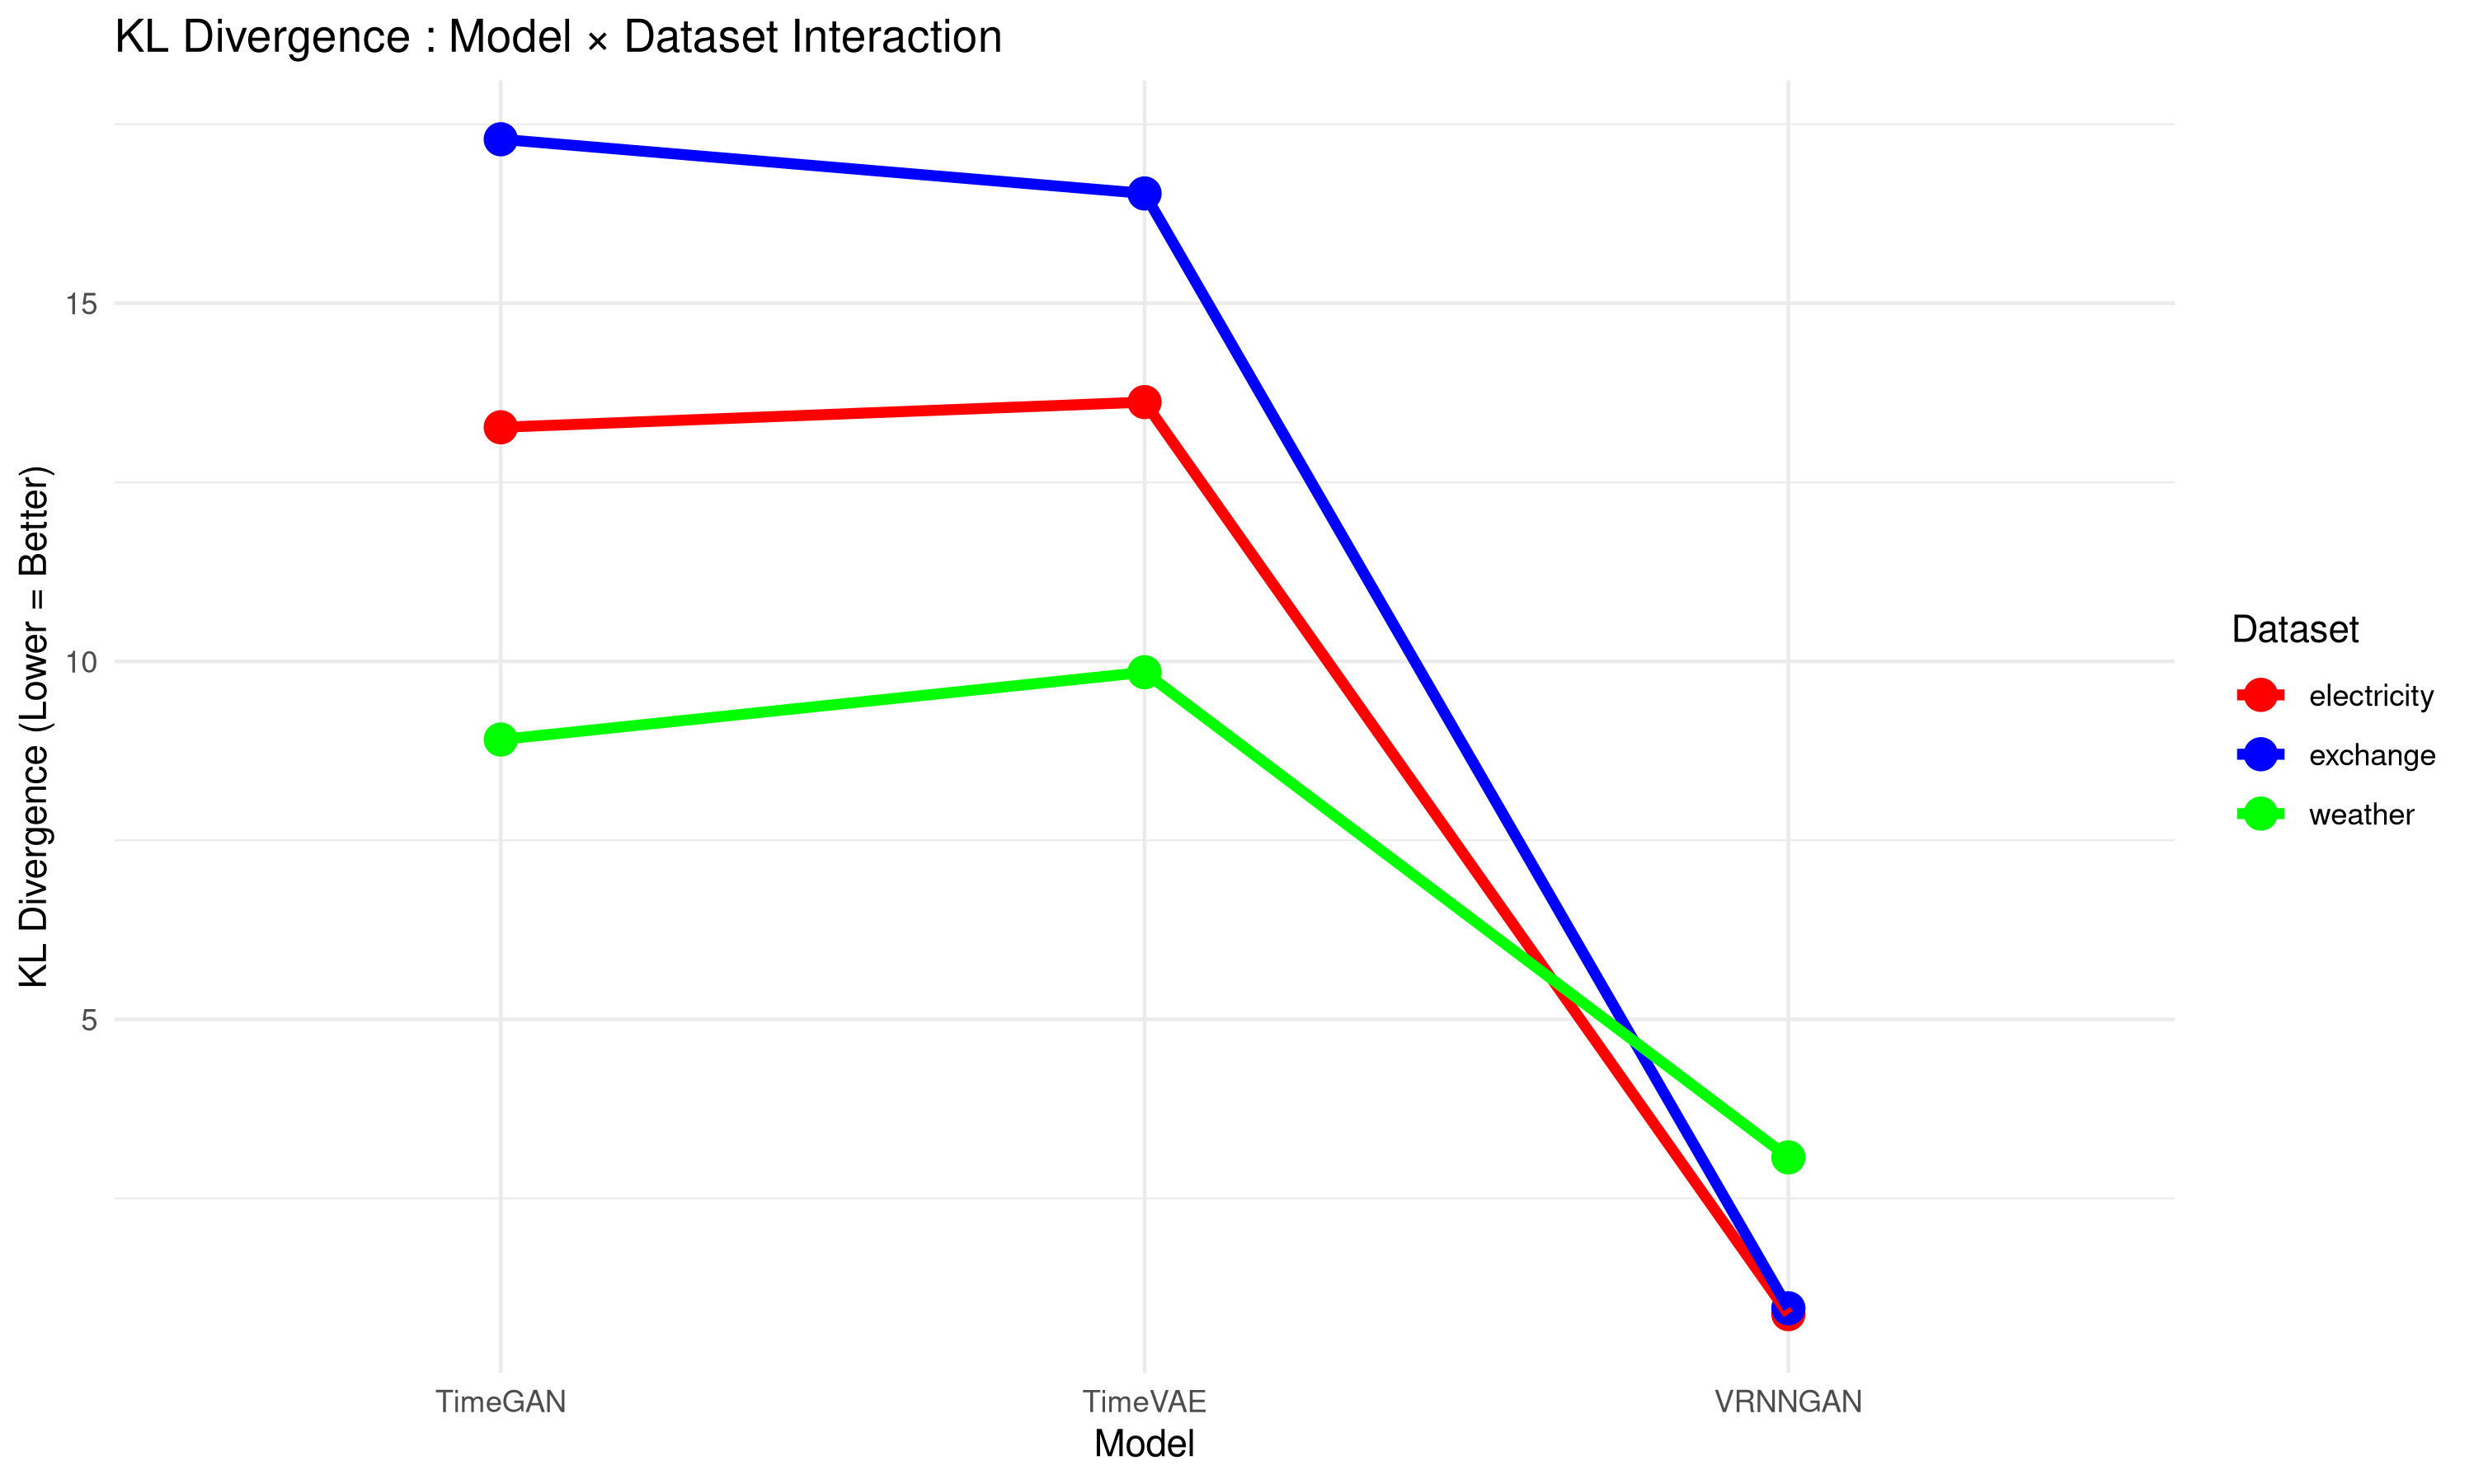
\includegraphics[width=0.8\textwidth]{assets/interaction_kl.png}
\caption{Model × Dataset interaction effects for KL Divergence}
\label{fig:kl_interaction}
\end{figure}

The Wasserstein distance interactions, shown in Figure \ref{fig:wasserstein_interaction}, reveal different patterns where TimeVAE demonstrates superior performance specifically for electricity data, while TimeGAN shows advantages for exchange data. These crossing lines exemplify how geometric similarity preservation varies significantly by dataset characteristics.

\begin{figure}[H]
\centering
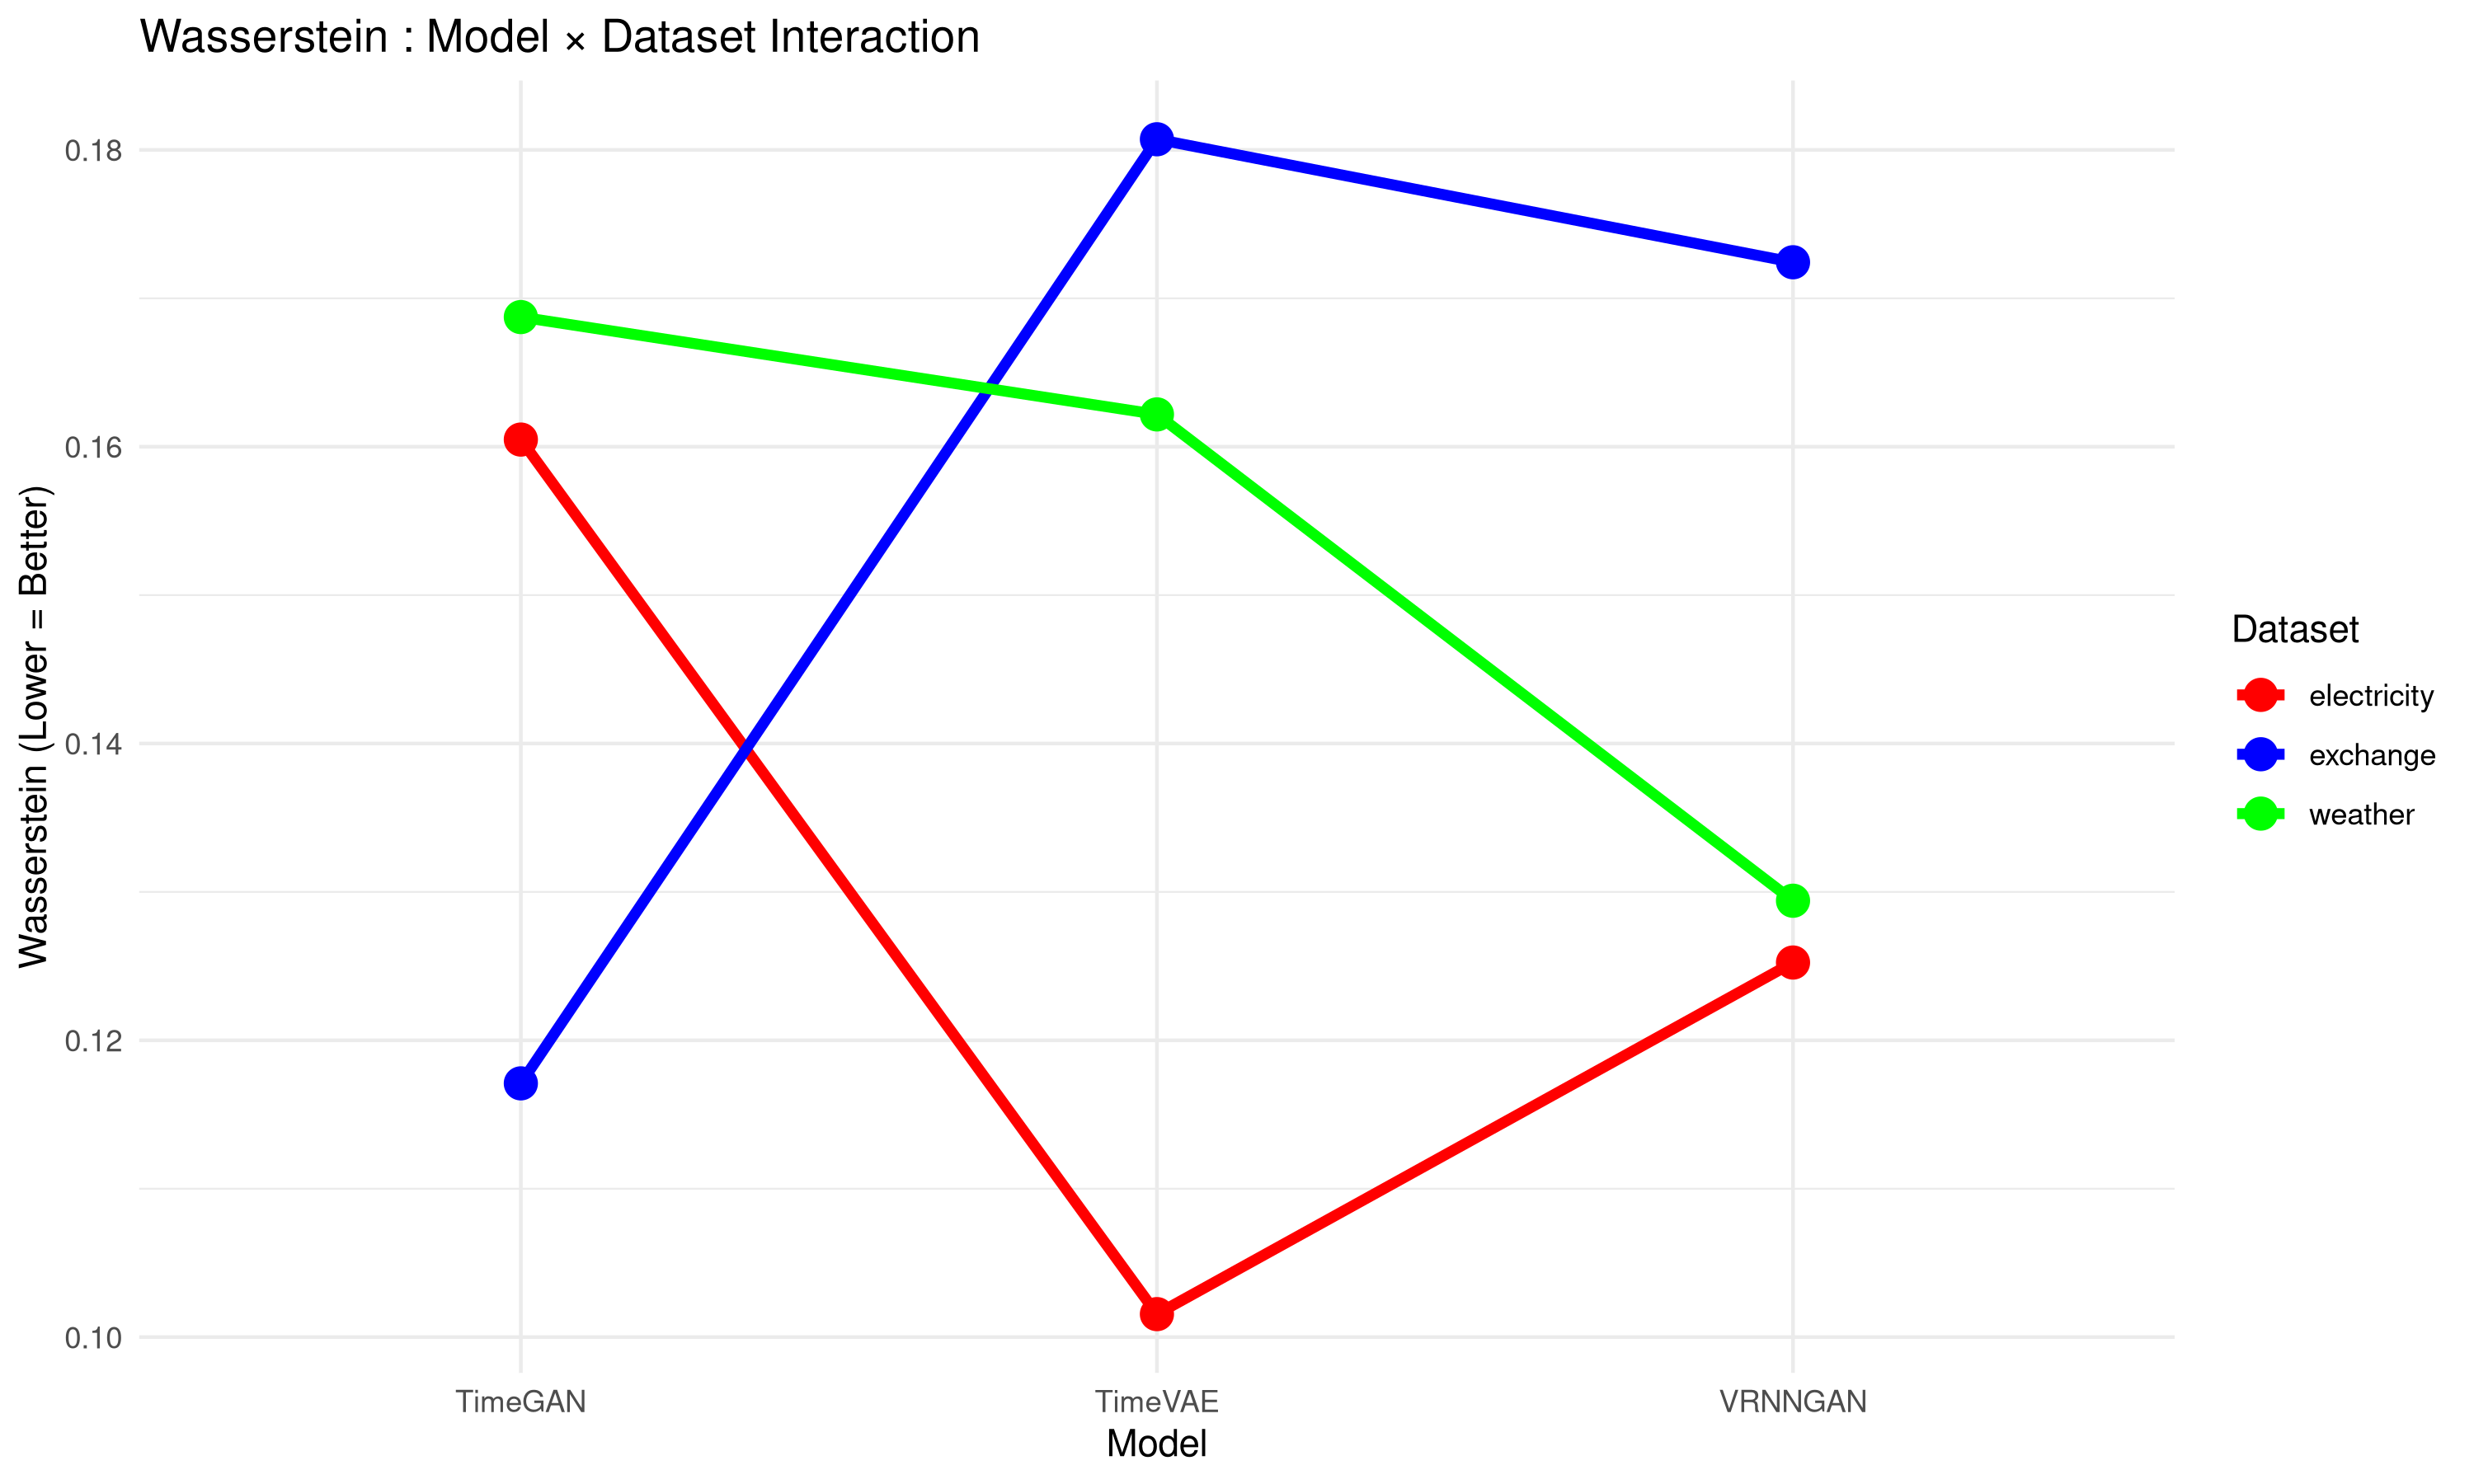
\includegraphics[width=0.8\textwidth]{assets/interaction_wasserstein.png}
\caption{Model × Dataset interaction effects for Wasserstein distance}
\label{fig:wasserstein_interaction}
\end{figure}

Figures \ref{fig:rmse_interaction} and \ref{fig:mae_interaction} display the forecasting performance interactions, where weather data presents unique challenges for all models, particularly affecting TimeVAE performance. The near-parallel lines for electricity and exchange data in both RMSE and MAE suggest more consistent relative model performance for these forecasting metrics across these datasets.

\begin{figure}[H]
\centering
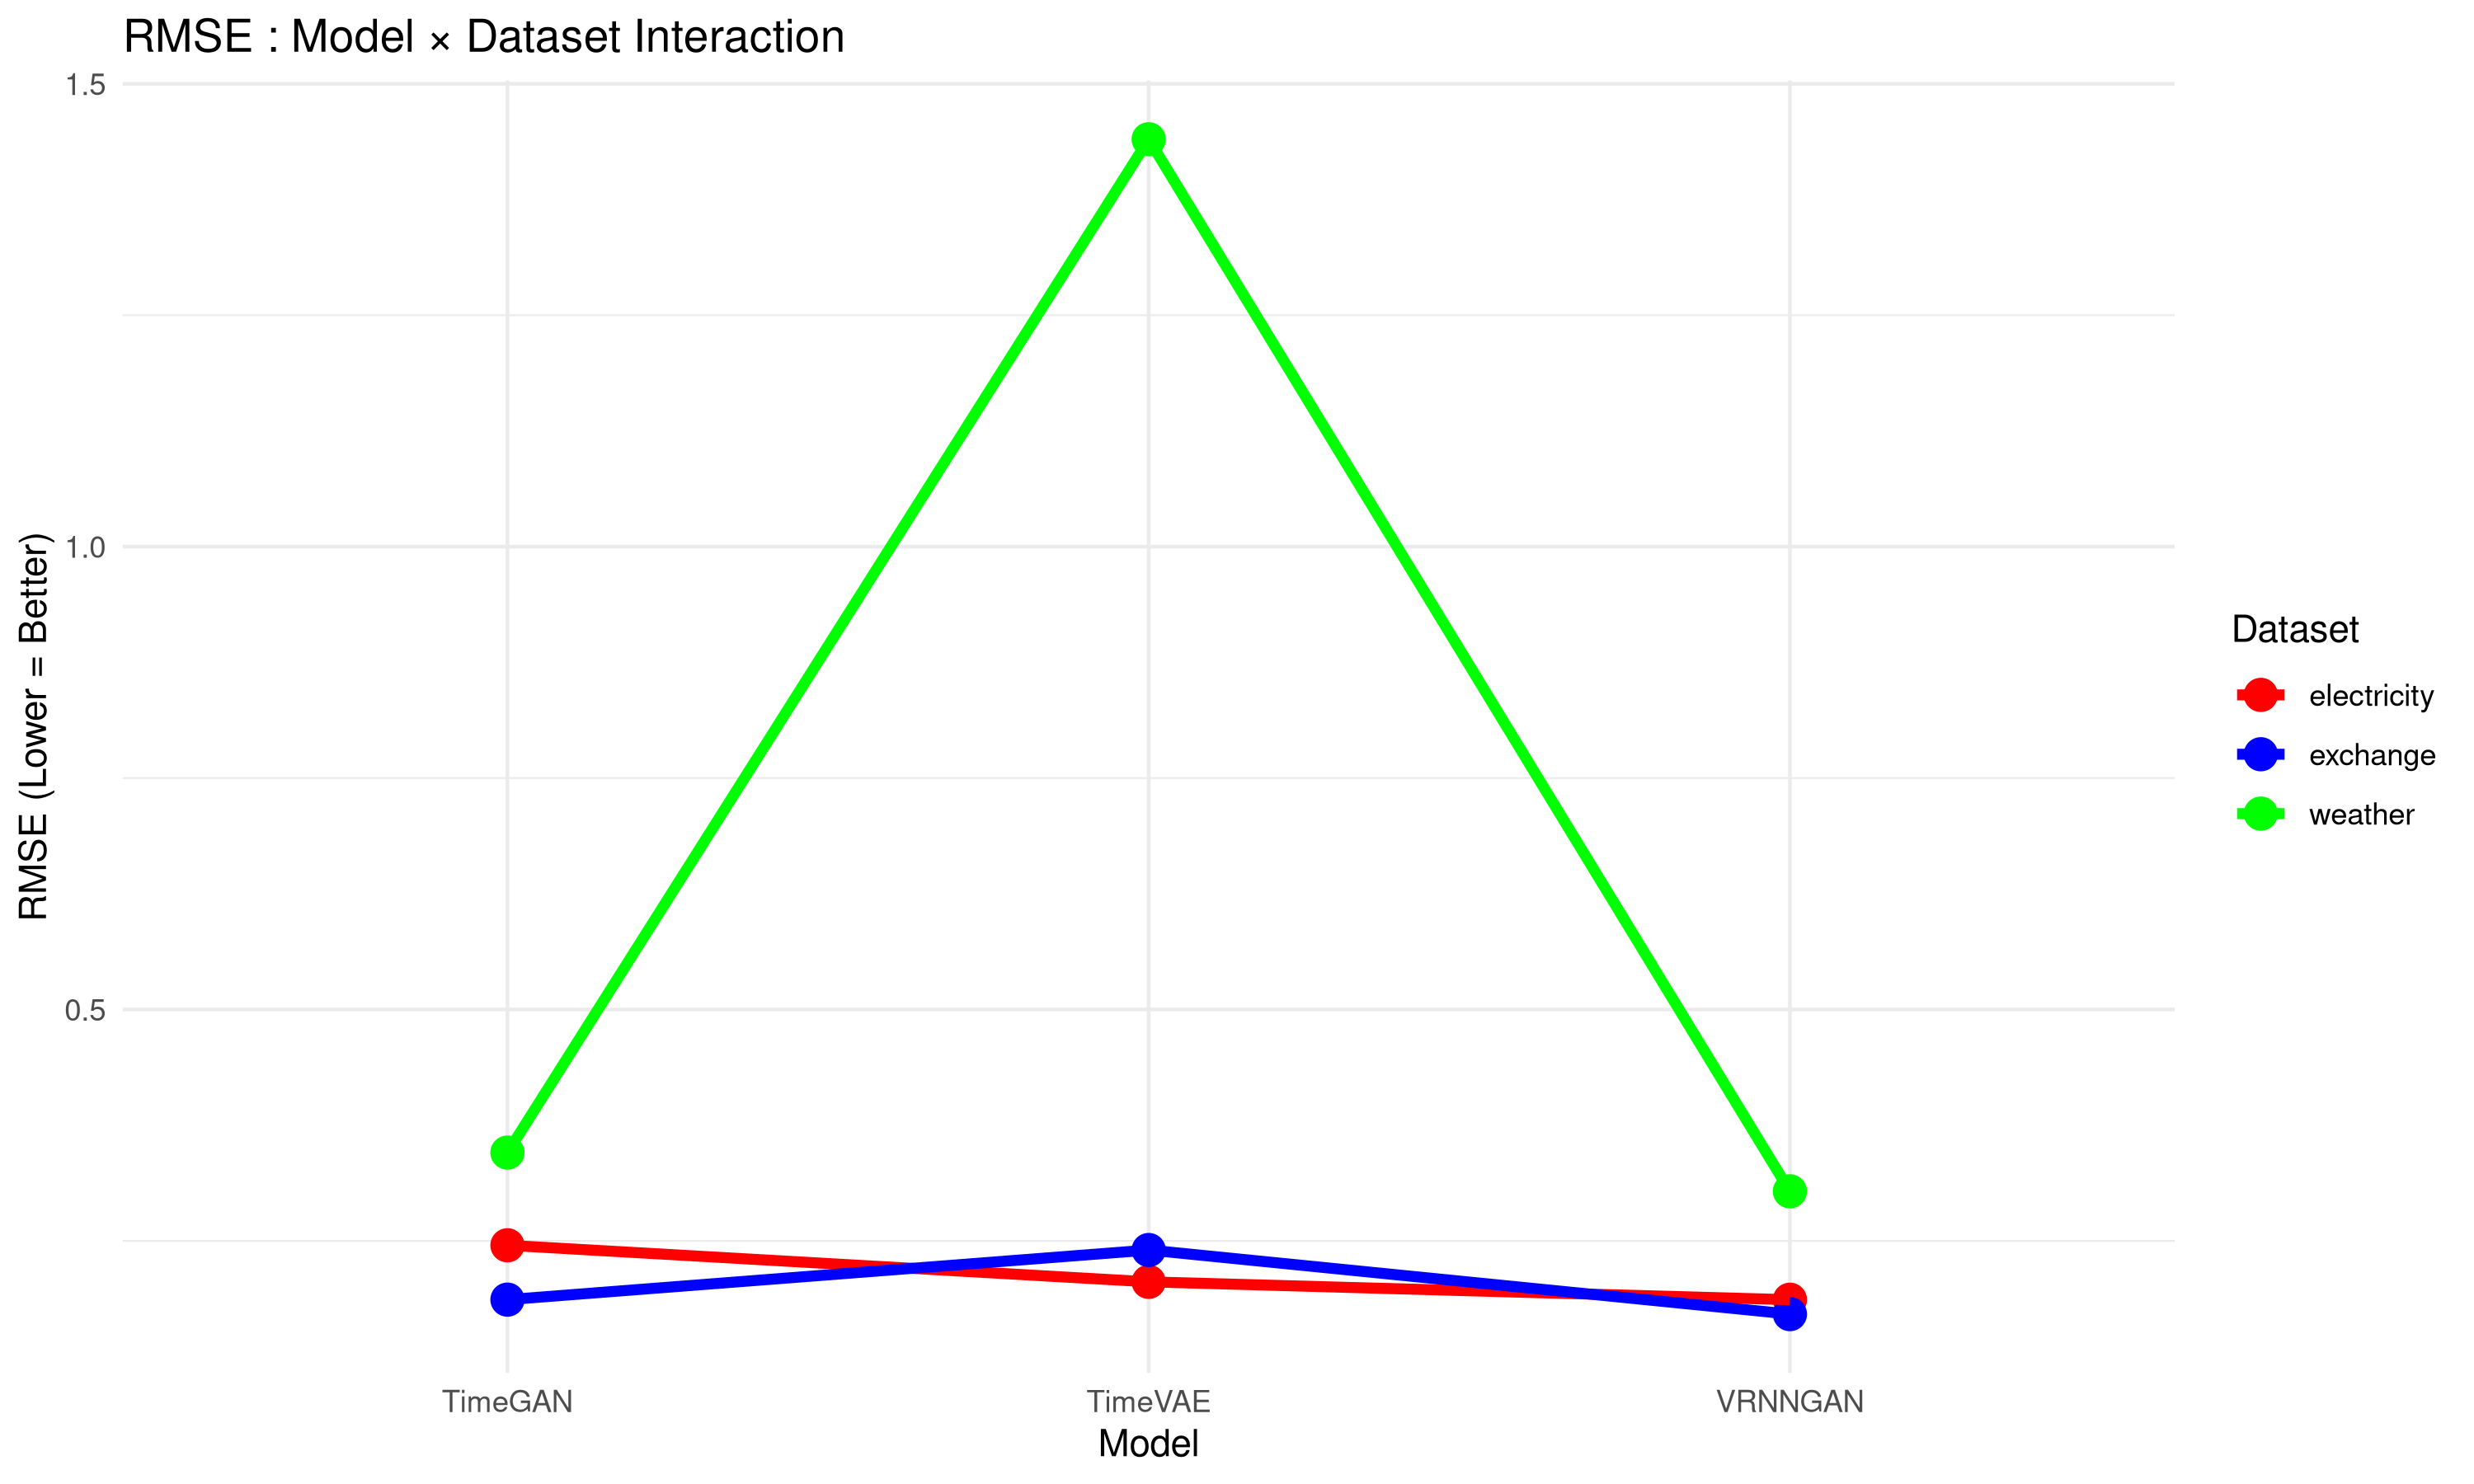
\includegraphics[width=0.8\textwidth]{assets/interaction_rmse.png}
\caption{Model × Dataset interaction effects for RMSE}
\label{fig:rmse_interaction}
\end{figure}

\begin{figure}[H]
\centering
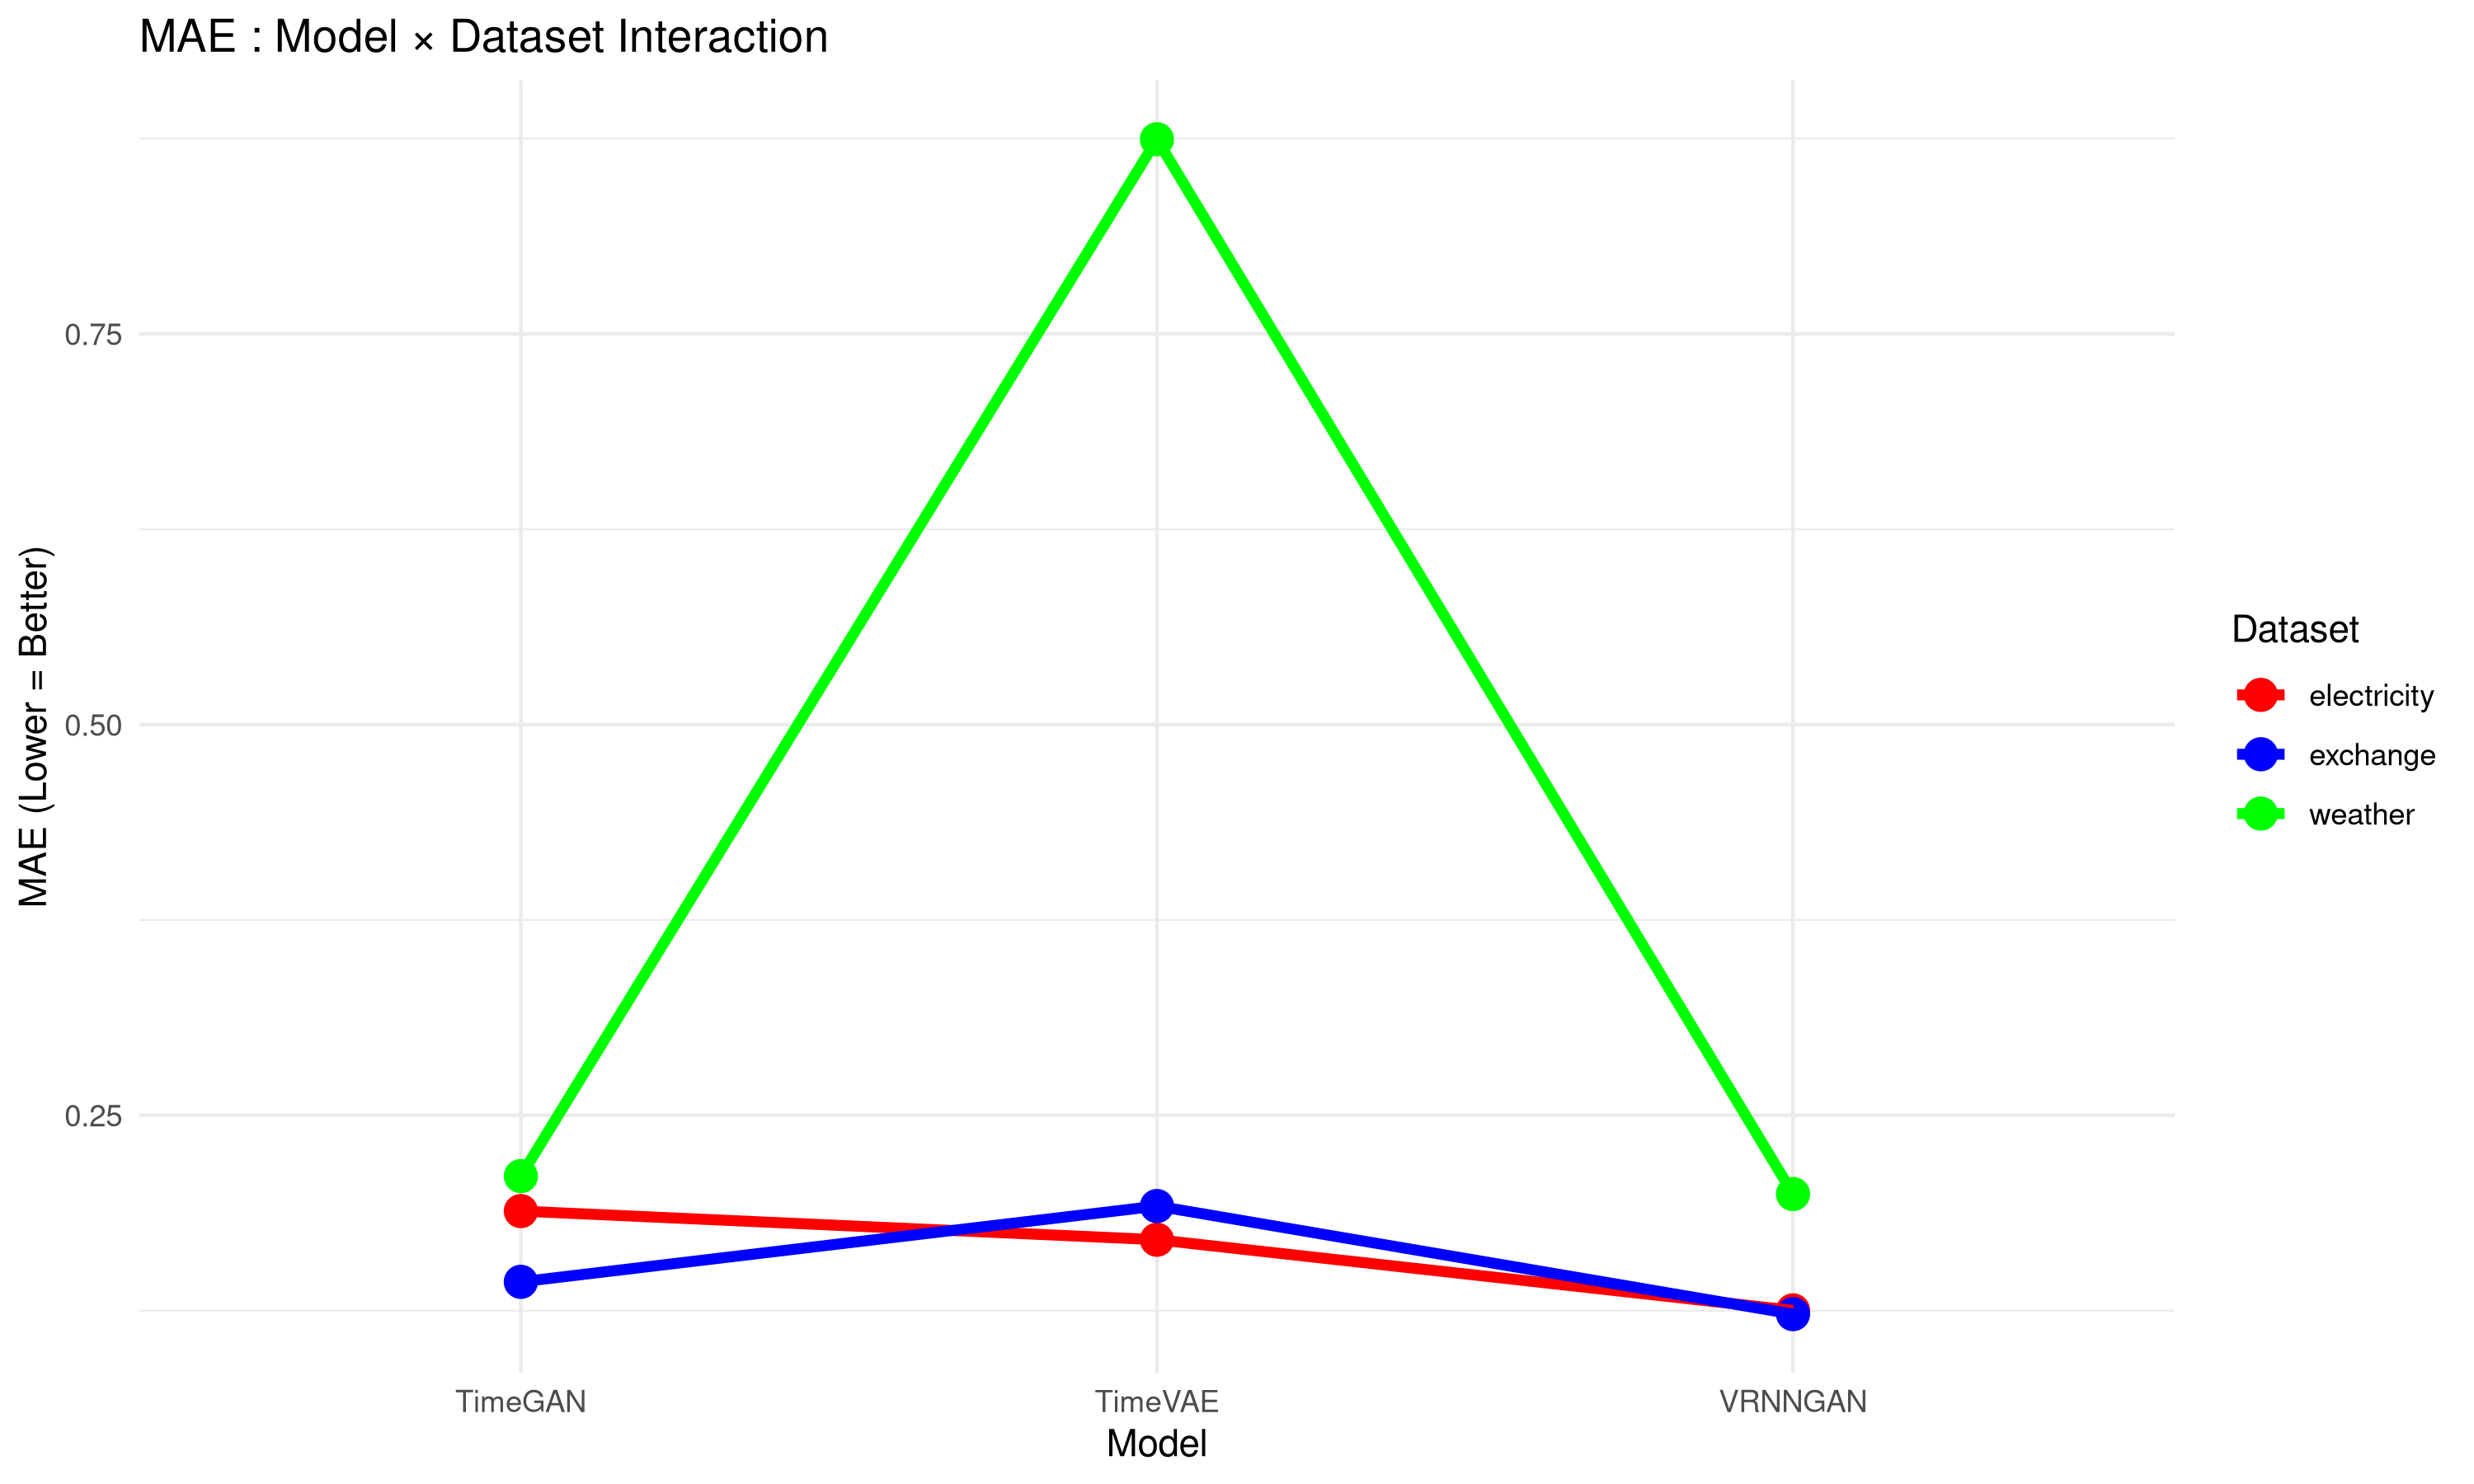
\includegraphics[width=0.8\textwidth]{assets/interaction_mae.png}
\caption{Model × Dataset interaction effects for MAE}
\label{fig:mae_interaction}
\end{figure}

These interaction patterns validate the statistical findings from the ANOVA analysis, demonstrating that model selection cannot be made universally but must consider the specific properties of the target dataset. The varying interaction strengths across metrics further indicate that different aspects of synthetic data quality—statistical fidelity versus forecasting utility—are affected differently by dataset characteristics, necessitating the dataset-specific Shapley analysis that follows.


\subsubsection{Tukey-HSD Post-Hoc Results}

Following the confirmation of statistically significant differences between models in the ANOVA analysis, Tukey HSD post-hoc tests were conducted to examine the specific patterns of these differences and identify exactly where the models differ from one another. This analysis provides detailed insights into the pairwise comparisons between TimeGAN, TimeVAE, and VRNNGAN across all evaluation metrics.

The post-hoc analysis reveals consistent performance hierarchies across metrics, with distinct groupings that highlight each model's relative strengths and weaknesses. For KL divergence (Table \ref{tab:tukey_kl}), which measures the divergence of synthetic data distributions from the real bootstrapped data distribution (serving as the reference), VRNNGAN demonstrates substantially superior performance with a mean value of 1.64, forming its own distinct group (c). TimeGAN and TimeVAE show relatively similar but significantly different performance levels, with TimeGAN (13.16, group a) slightly outperforming TimeVAE (13.33, group b). This pattern indicates that while both individual models struggle with statistical fidelity compared to the hybrid approach, TimeGAN maintains marginally better distributional similarity to the real reference data.
% KL Divergence Tukey HSD Results
\begin{table}[H]
\centering
\caption{Tukey HSD Post-Hoc Analysis for KL Divergence}
\label{tab:tukey_kl}
\begin{tabular}{lcc}
\toprule
\textbf{Model} & \textbf{Mean Value} & \textbf{Tukey Group} \\
\midrule
VRNNGAN & 1.6399 & c \\
TimeGAN & 13.1554 & a \\
TimeVAE & 13.3337 & b \\
\bottomrule
\end{tabular}
\footnotesize
\end{table}

The Wasserstein distance results (Table \ref{tab:tukey_wasserstein}) reveal a different performance ranking, where all three models form distinct statistical groups despite relatively small absolute differences. VRNNGAN again achieves the best performance (0.142, group c), followed by TimeVAE (0.148, group b) and TimeGAN (0.149, group a). The closer clustering of values suggests that geometric similarity preservation shows less dramatic differences between models compared to statistical divergence measures.

% Wasserstein Distance Tukey HSD Results
\begin{table}[H]
\centering
\caption{Tukey HSD Post-Hoc Analysis for Wasserstein Distance}
\label{tab:tukey_wasserstein}
\begin{tabular}{lcc}
\toprule
\textbf{Model} & \textbf{Mean Value} & \textbf{Tukey Group} \\
\midrule
VRNNGAN & 0.1424 & c \\
TimeVAE & 0.1481 & b \\
TimeGAN & 0.1488 & a \\
\bottomrule
\end{tabular}
\footnotesize
\end{table}

For forecasting performance metrics, the post-hoc analysis demonstrates more pronounced differences between models. In RMSE evaluation (Table \ref{tab:tukey_rmse}), VRNNGAN maintains its superior performance (0.220, group c), while TimeGAN (0.259, group a) significantly outperforms TimeVAE (0.629, group b). This substantial gap indicates that TimeVAE's approach to latent space modeling may not effectively capture the temporal dependencies necessary for accurate forecasting. Similarly, MAE results (Table \ref{tab:tukey_mae}) confirm this pattern, with VRNNGAN (0.149, group c) leading, followed by TimeGAN (0.181, group a), and TimeVAE showing notably higher error rates (0.412, group b).


% RMSE Tukey HSD Results
\begin{table}[H]
\centering
\caption{Tukey HSD Post-Hoc Analysis for RMSE}
\label{tab:tukey_rmse}
\begin{tabular}{lcc}
\toprule
\textbf{Model} & \textbf{Mean Value} & \textbf{Tukey Group} \\
\midrule
VRNNGAN & 0.2203 & c \\
TimeGAN & 0.2591 & a \\
TimeVAE & 0.6287 & b \\
\bottomrule
\end{tabular}
\footnotesize
\end{table}

% MAE Tukey HSD Results
\begin{table}[H]
\centering
\caption{Tukey HSD Post-Hoc Analysis for MAE}
\label{tab:tukey_mae}
\begin{tabular}{lcc}
\toprule
\textbf{Model} & \textbf{Mean Value} & \textbf{Tukey Group} \\
\midrule
VRNNGAN & 0.1492 & c \\
TimeGAN & 0.1811 & a \\
TimeVAE & 0.4123 & b \\
\bottomrule
\end{tabular}
\footnotesize
\end{table}

The consistent emergence of three distinct statistical groups across all metrics confirms that each model contributes unique characteristics to synthetic data generation. VRNNGAN's consistent placement in the superior performance group (c) across all metrics validates the effectiveness of hybrid architectures in balancing multiple aspects of data quality. The varying relative positions of TimeGAN and TimeVAE across different metrics highlight the trade-offs inherent in different generative approaches, with TimeGAN showing particular strength in forecasting tasks and TimeVAE demonstrating competitive performance in certain geometric similarity measures.

\subsection{Shapley Value Analysis}
The Shapley analysis reveals the individual contributions of each model component to the overall performance across different metrics and datasets. For each metric evaluated, the analysis examines the marginal contributions and interactions between model components.

% Dataset-Specific Shapley Analysis Summary

\begin{figure}[H]
\centering
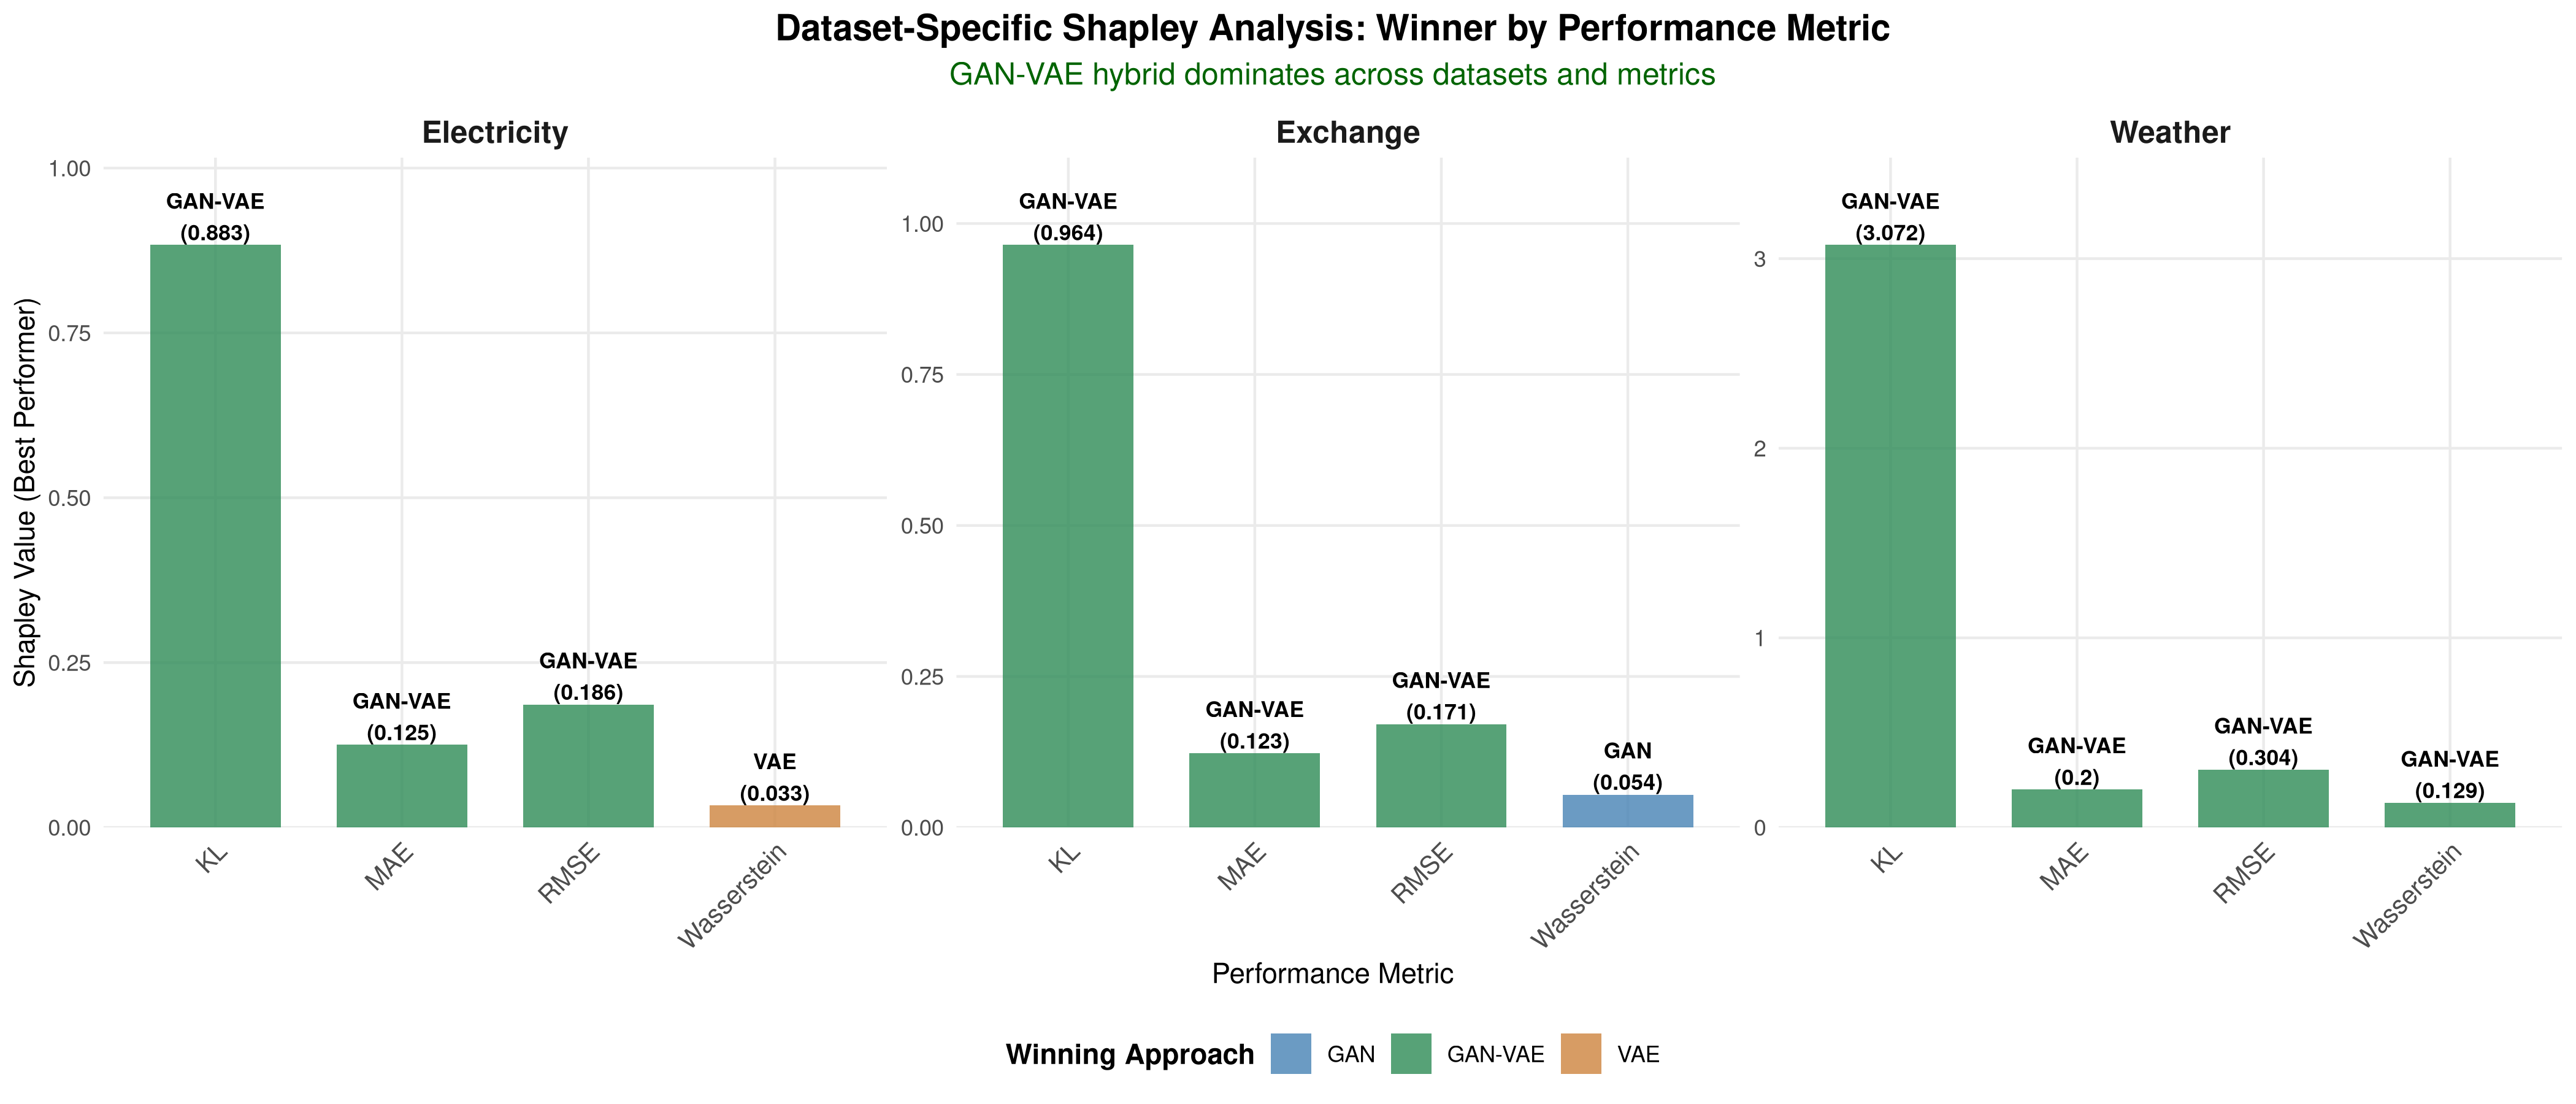
\includegraphics[width=0.8\textwidth]{assets/shapley_dataset_winners.png}
\caption{Shapley Analysis Summary Plot}
\label{fig:shap}
\end{figure}

The comprehensive analysis across datasets reveals distinct patterns in model effectiveness. VRNNGAN demonstrates consistent superiority across most metrics and datasets, with particularly strong performance in statistical fidelity measures (KL divergence) and forecasting accuracy (RMSE, MAE). However, individual models show dataset-specific advantages: TimeVAE excels in geometric similarity preservation for electricity data, while TimeGAN demonstrates superior Wasserstein distance performance for exchange data. 

\subsubsection{Electricity Dataset Results}

he electricity dataset demonstrates VRNNGAN's strong performance across most evaluation metrics, with the notable exception of Wasserstein distance where TimeVAE shows superior geometric similarity preservation. Table \ref{tab:shapley_electricity} shows that VRNNGAN achieves the highest Shapley values for KL divergence (0.883), RMSE (0.186), and MAE (0.125), indicating consistent effectiveness in both statistical fidelity and forecasting utility.
\begin{table}[H]
\centering
\caption{Shapley value contributions: electricity dataset}
\label{tab:shapley_electricity}
\begin{tabular}{lcccc}
\toprule
\textbf{Approach} & \textbf{KL Divergence} & \textbf{Wasserstein} & \textbf{RMSE} & \textbf{MAE} \\
\midrule
TimeGAN & 0.266 & 0.092 & 0.113 & 0.072 \\
TimeVAE & 0.618 & \textbf{0.033} & 0.073 & 0.053 \\
VRNNGAN & \textbf{0.883} & 0.125 & \textbf{0.186} & \textbf{0.125} \\
\bottomrule
\end{tabular}
\\[0.5em]
\footnotesize
\textit{Note: Bold indicates highest Shapley value (best contributor) per metric.}
\end{table}

\subsubsection{Exchange Dataset Results}
he exchange dataset analysis reveals VRNNGAN's dominance across most metrics, with notable exceptions in geometric similarity preservation. Table \ref{tab:shapley_exchange} demonstrates that for KL divergence, VRNNGAN achieves the highest Shapley value (0.964), indicating exceptional statistical fidelity preservation. However, TimeGAN demonstrates superior performance for Wasserstein distance (0.054), suggesting better geometric similarity modeling for this specific financial dataset context.

\begin{table}[H]
\centering
\caption{Shapley value contributions: exchange dataset}
\label{tab:shapley_exchange}
\begin{tabular}{lcccc}
\toprule
\textbf{Approach} & \textbf{KL Divergence} & \textbf{Wasserstein} & \textbf{RMSE} & \textbf{MAE} \\
\midrule
TimeGAN & 0.861 & \textbf{0.054} & 0.059 & 0.037 \\
TimeVAE & 0.104 & 0.118 & 0.112 & 0.086 \\
VRNNGAN & \textbf{0.964} & 0.172 & \textbf{0.171} & \textbf{0.123} \\
\bottomrule
\end{tabular}
\\[0.5em]
\footnotesize
\textit{Note: Bold indicates highest Shapley value (best contributor) per metric.}
\end{table}

\subsubsection{Weather Dataset Results}
he weather dataset presents the most challenging context for synthetic data generation, evidenced by the emergence of negative Shapley contributions. Table \ref{tab:shapley_weather} reveals that VRNNGAN maintains superior performance across all metrics, with particularly strong contributions for KL divergence (3.072). Notably, TimeGAN exhibits negative contributions for RMSE (-0.396) and MAE (-0.232), indicating that its inclusion in coalition modeling actually degrades forecasting performance for this complex meteorological dataset.

\begin{table}[H]
\centering
\caption{Shapley value contributions: weather dataset}
\label{tab:shapley_weather}
\begin{tabular}{lcccc}
\toprule
\textbf{Approach} & \textbf{KL Divergence} & \textbf{Wasserstein} & \textbf{RMSE} & \textbf{MAE} \\
\midrule
TimeGAN & 1.066 & 0.068 & -0.396 & -0.232 \\
TimeVAE & 2.006 & 0.061 & 0.699 & 0.432 \\
VRNNGAN & \textbf{3.072} & \textbf{0.129} & \textbf{0.304} & \textbf{0.200} \\
\bottomrule
\end{tabular}
\\[0.5em]
\footnotesize
\textit{Note: Bold indicates highest Shapley value (best contributor) per metric. Negative values indicate performance degradation when model is included.}
\end{table}


\subsection{Discussion}
\newpage
\section{CONCLUSION AND FUTURE WORKS}
This study explores the application of Shapley value analysis to evaluate generative models for synthetic time series data generation, focusing on the balance between fidelity and usability metrics. The research systematically compared TimeGAN, TimeVAE, and VRNNGAN across three diverse datasets to determine optimal model selection strategies for synthetic data applications. 

The methodology employed a comprehensive evaluation framework that integrated statistical fidelity measures and forecasting utility metrics within a Shapley-based analysis system. Bootstrap validation provided statistical robustness, while ANOVA analysis confirmed significant model-dataset interactions across all evaluation metrics.

The results demonstrate VRNNGAN's consistent superiority across all evaluation scenarios. The hybrid model achieved the highest performance in both distributional similarity and forecasting accuracy, with substantial improvements over individual model approaches. Model effectiveness varied considerably across different time series characteristics, with hybrid advantages ranging significantly depending on context. 

These findings contribute to the body of knowledge by establishing Shapley value analysis as a mathematically principled framework for interpretable evaluation of generative models, moving beyond traditional comparative approaches to fair attribution of model contributions. The research advances understanding of how different generative architectures create value in synthetic data generation through systematic decomposition of performance contributions. For practitioners, this work provides empirical evidence for hybrid architecture superiority in balancing multiple quality dimensions and demonstrates the importance of context-aware model selection rather than universal benchmarking approaches in real-world synthetic data applications.

The study's limitations include its focus on forecasting tasks using LSTM networks, which may not generalize to other machine learning applications such as classification or anomaly detection. The deliberate exclusion of privacy metrics represents a significant limitation given the critical importance of privacy preservation in synthetic data applications. Additionally, the evaluation scope was constrained to time series data and three specific datasets, which may not capture the full diversity of real-world data characteristics.

Due to the lack of comprehensive privacy evaluation in this framework, future scholars can extend the Shapley-based analysis to incorporate differential privacy metrics, creating a three-dimensional evaluation ecosystem that addresses fidelity, usability, and privacy simultaneously. Future research should explore the framework's applicability to diverse machine learning tasks beyond forecasting and investigate the specific data characteristics that drive the observed model-dataset interactions. Additionally, scaling studies with larger datasets and emerging generative architectures would further validate the framework's broader applicability.



\newpage

\begin{center}
\Large\textbf{DECLARATION OF CONFLICTS OF INTEREST}
\end{center}

\vspace{1em} % adds a little vertical space

The author declares that there is no conflict of interest regarding the publication of this paper.

\newpage

\begin{center}
\Large\textbf{DATA AVAILABILITY}
\end{center}

\vspace{1em} % adds a little vertical space

The data used in this study were sourced from PapersWithCode.

% Include all references, even if they are not cited in the text
\nocite{*}

% Print the bibliography
% \printbibliography
\end{document}